\documentclass[11pt]{article}

\usepackage[margin=1in]{geometry}
\usepackage{amsmath,amssymb,amsthm}
\usepackage{mathtools}
\usepackage{graphicx}
\usepackage{booktabs}
\usepackage{array}
\usepackage{microtype}
\usepackage{tikz}
\usepackage[shortlabels]{enumitem}
\usepackage[colorlinks=true,linkcolor=blue!45!black,citecolor=blue!45!black,urlcolor=blue!45!black]{hyperref}

% ---------- colors for the two maps (as in the paper on Problem 137) ----------
\definecolor{fred}{RGB}{178,58,46}
\definecolor{gblue}{RGB}{51,96,143}

% ---------- theorem environments ----------
\newtheorem{theorem}{Theorem}[section]
\newtheorem{lemma}[theorem]{Lemma}
\newtheorem{proposition}[theorem]{Proposition}
\newtheorem{corollary}[theorem]{Corollary}
\newtheorem{conjecture}[theorem]{Conjecture}
\theoremstyle{definition}
\newtheorem{definition}[theorem]{Definition}
\newtheorem{example}[theorem]{Example}
\newtheorem{question}[theorem]{Question}
\theoremstyle{remark}
\newtheorem{remark}[theorem]{Remark}
\newtheorem*{thmA}{Theorem A$_q$}
\newtheorem*{thmB}{Theorem B$_q$}
\newtheorem*{thmC}{Theorem C$_q$}
\newtheorem*{thmD}{Theorem D}
\newtheorem*{thmE}{Theorem E}

% ---------- notation ----------
\newcommand{\Q}{\mathbb{Q}}
\newcommand{\Z}{\mathbb{Z}}
\newcommand{\R}{\mathbb{R}}
\newcommand{\Orb}{\mathcal{O}}
\newcommand{\Term}{\mathcal{T}}
\newcommand{\rf}[1]{[#1]_{\lambda}}
\newcommand{\hj}[1]{[#1]^{-}}
\newcommand{\old}[2]{\textcolor{black!50}{#1}_{\textcolor{black!50}{[#2]}}}

\tikzset{
  vpos/.style={draw=fred,fill=fred!8,rounded corners=2.5pt,inner xsep=2pt,inner ysep=1.5pt},
  vneg/.style={draw=gblue,fill=gblue!8,rounded corners=2.5pt,inner xsep=2pt,inner ysep=1.5pt},
  vroot/.style={draw=black!70,fill=black!6,rounded corners=2.5pt,inner xsep=2pt,inner ysep=1.5pt},
  rk/.style={font=\tiny,text=black!55},
  ef/.style={draw=fred!75,thick},
  eg/.style={draw=gblue!75,thick},
  eold/.style={->,>=stealth,densely dashed,draw=black!40,semithick},
}

\title{Why three? Trees of rationals from $x\mapsto x+1$ and an involution}
\author{Arjun Pemmasani\\
\textit{[Placeholder for the author: affiliation and email address]}}
\date{}

\begin{document}
\maketitle

\begin{abstract}
Start at $0$ and apply the maps $x\mapsto x+1$ and $x\mapsto-1/x$. Problem 137 of Kagey's Open Problem
Collection asks why the number $a(n)$ of rationals first reached after $n$ steps satisfies
$a(n)=a(n-1)+a(n-3)$. We show that the $3$ is the order of the map $x\mapsto-1/(x+1)$. To see this we
replace $-1/x$ by $g_m(x)=-1/(mx)$. For $m=2$ and $m=3$ the composite $g_m(x+1)$ has order $q=4$ and
$q=6$, every rational is still reached, and the counts satisfy
$a(n)=a(n-1)+a(n-3)+\dots+a(n-2q+3)$ for $n\ge 2q-2$. More generally, for every $q\ge3$ the tree of
$X\mapsto X+2\cos(\pi/q)$ and $X\mapsto-1/X$ has rank generating function
$(1+t^2+\dots+t^{2q-4}-t^{2q-3})/(1-t-t^3-\dots-t^{2q-3})$. The proof gives the rank of each point
from a continued fraction whose digits obey one rule. No $q-2$ digits in a row after the first may
equal $1$, with one exception at the root. For
$m\ge4$ the composite has infinite order, the counts are Fibonacci numbers, and some rationals are
never reached.
\end{abstract}

\noindent\textbf{2020 Mathematics Subject Classification:} 11B37, 05A15, 11A55, 20H10.

\noindent\textbf{Keywords:} tree of rationals, linear recurrence, Hecke group, Rosen continued
fraction, generating function.

\section{Introduction}\label{sec:intro}

\subsection{The question}

Let $f(x)=x+1$ and $g(x)=-1/x$. Start at $0$ and apply $f$ and $g$ in any order, never applying $g$
to $0$. Every rational is reached, and the \emph{rank} of a rational is the least number of moves
needed to reach it. Kimberling sorted the rationals by rank in OEIS A226247 \cite{oeisA226247}, and
Kagey asked whether the number $a(n)$ of rationals of rank $n$ satisfies $a(n)=a(n-1)+a(n-3)$
\cite{kagey-mse,kagey137}. In earlier work \cite{P137} we proved this for $n\ge4$, together with a
formula for the rank and a description of the tree. Kimberling and Moses had stated the same
recurrence for the version of the tree with root $1$ \cite[Example~4.2]{kimberling-moses}.

This paper asks where the $3$ comes from. The answer is short. The map
\[
g(f(x))=-\frac{1}{x+1}
\]
has order $3$, since $x\mapsto-1/(x+1)\mapsto-(x+1)/x\mapsto x$. To test this reading we change $g$
so that $g\circ f$ has a different order and see what happens to the recurrence. Keep $f(x)=x+1$ and
the root $0$, and for an integer $m\ge1$ put
\[
g_m(x)=-\frac{1}{mx}.
\]
Problem 137 is the case $m=1$. The composite $g_m(f(x))=-1/(m(x+1))$ is a M\"obius map with
trace $m$ and determinant $m$. It has order $3$, $4$ and $6$ for $m=1$, $2$ and $3$, and infinite
order for $m\ge4$ (Lemma~\ref{lem:order}). We write $q$ for this order. Table~\ref{tab:family}
summarizes what we prove about each case.

\begin{table}[ht]
\centering\small
\renewcommand{\arraystretch}{1.15}
\begin{tabular}{@{}c c c l l@{}}
\toprule
$m$ & $q$ & points of the tree & generating function of $a(n)$ & recurrence\\
\midrule
$1$ & $3$ & all of $\Q$ & $\dfrac{1+t^2-t^3}{1-t-t^3}$ & $a(n)=a(n-1)+a(n-3)$, $n\ge4$\\[8pt]
$2$ & $4$ & all of $\Q$ & $\dfrac{1+t^2+t^4-t^5}{1-t-t^3-t^5}$ & $a(n)=a(n-1)+a(n-3)+a(n-5)$, $n\ge6$\\[8pt]
$3$ & $6$ & all of $\Q$ & $\dfrac{1+t^2+t^4+t^6+t^8-t^9}{1-t-t^3-t^5-t^7-t^9}$ &
  $a(n)=\sum_{j=0}^{4}a(n-2j-1)$, $n\ge10$\\[8pt]
$\ge4$ & $\infty$ & not all of $\Q$ & $\dfrac{1}{1-t-t^2}$ & $a(n)=a(n-1)+a(n-2)$, $n\ge2$\\
\bottomrule
\end{tabular}
\caption{The trees of $f(x)=x+1$ and $g_m(x)=-1/(mx)$ with root $0$. The row $m=1$ is
\cite{P137}. In the third row the sum is $a(n-1)+a(n-3)+a(n-5)+a(n-7)+a(n-9)$. For $m\le3$ each
recurrence fails at the first $n$ below the stated range.}
\label{tab:family}
\end{table}

So the $3$ in Problem 137 is the order of $g\circ f$, and the recurrence for order $q$ has the
$q-1$ lags $1,3,5,\dots,2q-3$. The family also shows why the more obvious generalization
$x\mapsto x+k$ with $x\mapsto-1/x$ is not interesting. Putting $x=ky$ turns it into the tree of
$y\mapsto y+1$ and $y\mapsto-1/(k^2y)$, which is the case $m=k^2\ge4$, and its counts are
Fibonacci numbers.

The cases $m=2$ and $m=3$ give new trees of rationals. They are the only other values of $m$ for
which the tree is all of $\Q$ (Theorem~D and Theorem~E). Their counts start
\begin{align*}
(m=2)&\qquad 1, 1, 2, 3, 5, 7, 11, 18, 28, 44, 69, 108, 170, 267, 419, 658, 1033, \dots,\\
(m=3)&\qquad 1, 1, 2, 3, 5, 8, 13, 21, 34, 54, 87, 141, 227, 366, 590, 951, 1533, \dots,
\end{align*}
and neither sequence is in the OEIS. Figure~\ref{fig:trees} shows the first ranks of the trees for
$m=1$ and $m=2$.

\begin{figure}[p]
\centering
\resizebox{0.86\textwidth}{!}{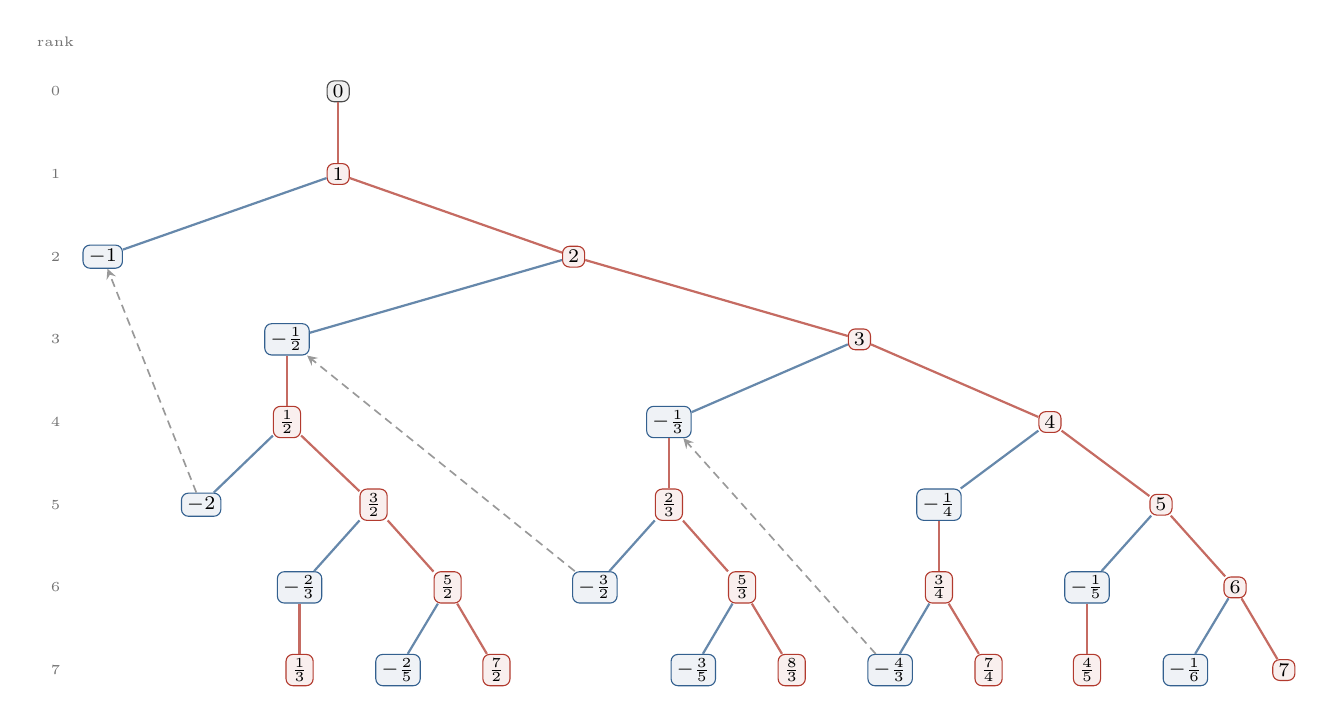
\begin{tikzpicture}[every node/.style={font=\scriptsize}]
\node[vroot] (n0_1) at (2.99,0.00) {$0$};
\node[vpos] (n1_1) at (2.99,-1.05) {$1$};
\node[vneg] (nm1_1) at (0.00,-2.10) {$-1$};
\node[vpos] (n2_1) at (5.98,-2.10) {$2$};
\node[vneg] (nm1_2) at (2.34,-3.15) {$-\tfrac{1}{2}$};
\node[vpos] (n3_1) at (9.61,-3.15) {$3$};
\node[vpos] (n1_2) at (2.34,-4.20) {$\tfrac{1}{2}$};
\node[vneg] (nm1_3) at (7.19,-4.20) {$-\tfrac{1}{3}$};
\node[vpos] (n4_1) at (12.03,-4.20) {$4$};
\node[vneg] (nm2_1) at (1.25,-5.25) {$-2$};
\node[vpos] (n3_2) at (3.44,-5.25) {$\tfrac{3}{2}$};
\node[vpos] (n2_3) at (7.19,-5.25) {$\tfrac{2}{3}$};
\node[vneg] (nm1_4) at (10.62,-5.25) {$-\tfrac{1}{4}$};
\node[vpos] (n5_1) at (13.44,-5.25) {$5$};
\node[vneg] (nm2_3) at (2.50,-6.30) {$-\tfrac{2}{3}$};
\node[vpos] (n5_2) at (4.38,-6.30) {$\tfrac{5}{2}$};
\node[vneg] (nm3_2) at (6.25,-6.30) {$-\tfrac{3}{2}$};
\node[vpos] (n5_3) at (8.12,-6.30) {$\tfrac{5}{3}$};
\node[vpos] (n3_4) at (10.62,-6.30) {$\tfrac{3}{4}$};
\node[vneg] (nm1_5) at (12.50,-6.30) {$-\tfrac{1}{5}$};
\node[vpos] (n6_1) at (14.38,-6.30) {$6$};
\node[vpos] (n1_3) at (2.50,-7.35) {$\tfrac{1}{3}$};
\node[vneg] (nm2_5) at (3.75,-7.35) {$-\tfrac{2}{5}$};
\node[vpos] (n7_2) at (5.00,-7.35) {$\tfrac{7}{2}$};
\node[vneg] (nm3_5) at (7.50,-7.35) {$-\tfrac{3}{5}$};
\node[vpos] (n8_3) at (8.75,-7.35) {$\tfrac{8}{3}$};
\node[vneg] (nm4_3) at (10.00,-7.35) {$-\tfrac{4}{3}$};
\node[vpos] (n7_4) at (11.25,-7.35) {$\tfrac{7}{4}$};
\node[vpos] (n4_5) at (12.50,-7.35) {$\tfrac{4}{5}$};
\node[vneg] (nm1_6) at (13.75,-7.35) {$-\tfrac{1}{6}$};
\node[vpos] (n7_1) at (15.00,-7.35) {$7$};
\node[rk] at (-0.6,0.63) {rank};
\node[rk] at (-0.6,0.00) {0};
\node[rk] at (-0.6,-1.05) {1};
\node[rk] at (-0.6,-2.10) {2};
\node[rk] at (-0.6,-3.15) {3};
\node[rk] at (-0.6,-4.20) {4};
\node[rk] at (-0.6,-5.25) {5};
\node[rk] at (-0.6,-6.30) {6};
\node[rk] at (-0.6,-7.35) {7};
\draw[ef] (n0_1) -- (n1_1);
\draw[eg] (n1_1) -- (nm1_1);
\draw[ef] (n1_1) -- (n2_1);
\draw[eg] (n2_1) -- (nm1_2);
\draw[ef] (n2_1) -- (n3_1);
\draw[ef] (nm1_2) -- (n1_2);
\draw[eg] (n3_1) -- (nm1_3);
\draw[ef] (n3_1) -- (n4_1);
\draw[eg] (n1_2) -- (nm2_1);
\draw[ef] (n1_2) -- (n3_2);
\draw[ef] (nm1_3) -- (n2_3);
\draw[eg] (n4_1) -- (nm1_4);
\draw[ef] (n4_1) -- (n5_1);
\draw[eg] (n3_2) -- (nm2_3);
\draw[ef] (n3_2) -- (n5_2);
\draw[eg] (n2_3) -- (nm3_2);
\draw[ef] (n2_3) -- (n5_3);
\draw[ef] (nm1_4) -- (n3_4);
\draw[eg] (n5_1) -- (nm1_5);
\draw[ef] (n5_1) -- (n6_1);
\draw[ef] (nm2_3) -- (n1_3);
\draw[eg] (n5_2) -- (nm2_5);
\draw[ef] (n5_2) -- (n7_2);
\draw[eg] (n5_3) -- (nm3_5);
\draw[ef] (n5_3) -- (n8_3);
\draw[eg] (n3_4) -- (nm4_3);
\draw[ef] (n3_4) -- (n7_4);
\draw[ef] (nm1_5) -- (n4_5);
\draw[eg] (n6_1) -- (nm1_6);
\draw[ef] (n6_1) -- (n7_1);
\draw[eold] (nm2_1) -- (nm1_1);
\draw[eold] (nm3_2) -- (nm1_2);
\draw[eold] (nm4_3) -- (nm1_3);
\end{tikzpicture}
}

\medskip
{\small (a) $m=1$, the tree of Problem 137.}

\bigskip
\resizebox{\textwidth}{!}{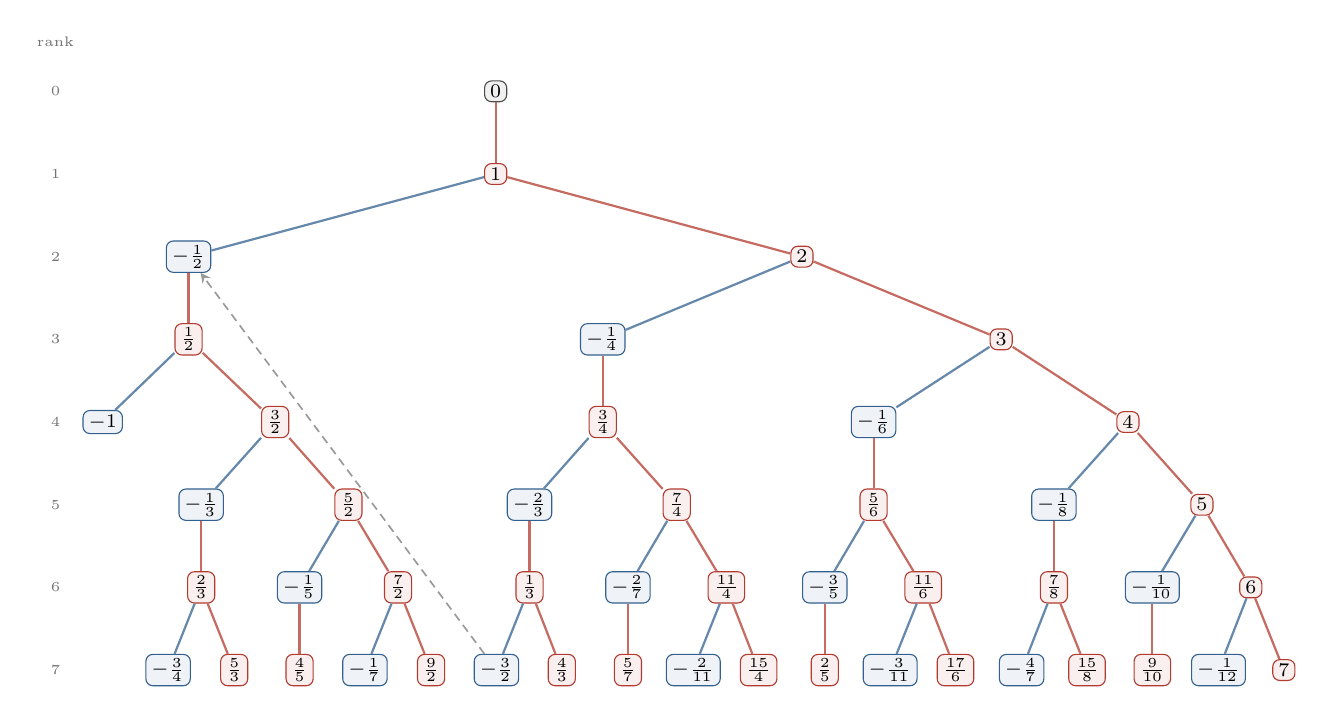
\begin{tikzpicture}[every node/.style={font=\scriptsize}]
\node[vroot] (n0_1) at (4.99,0.00) {$0$};
\node[vpos] (n1_1) at (4.99,-1.05) {$1$};
\node[vneg] (nm1_2) at (1.09,-2.10) {$-\tfrac{1}{2}$};
\node[vpos] (n2_1) at (8.88,-2.10) {$2$};
\node[vpos] (n1_2) at (1.09,-3.15) {$\tfrac{1}{2}$};
\node[vneg] (nm1_4) at (6.35,-3.15) {$-\tfrac{1}{4}$};
\node[vpos] (n3_1) at (11.41,-3.15) {$3$};
\node[vneg] (nm1_1) at (0.00,-4.20) {$-1$};
\node[vpos] (n3_2) at (2.19,-4.20) {$\tfrac{3}{2}$};
\node[vpos] (n3_4) at (6.35,-4.20) {$\tfrac{3}{4}$};
\node[vneg] (nm1_6) at (9.79,-4.20) {$-\tfrac{1}{6}$};
\node[vpos] (n4_1) at (13.02,-4.20) {$4$};
\node[vneg] (nm1_3) at (1.25,-5.25) {$-\tfrac{1}{3}$};
\node[vpos] (n5_2) at (3.12,-5.25) {$\tfrac{5}{2}$};
\node[vneg] (nm2_3) at (5.42,-5.25) {$-\tfrac{2}{3}$};
\node[vpos] (n7_4) at (7.29,-5.25) {$\tfrac{7}{4}$};
\node[vpos] (n5_6) at (9.79,-5.25) {$\tfrac{5}{6}$};
\node[vneg] (nm1_8) at (12.08,-5.25) {$-\tfrac{1}{8}$};
\node[vpos] (n5_1) at (13.96,-5.25) {$5$};
\node[vpos] (n2_3) at (1.25,-6.30) {$\tfrac{2}{3}$};
\node[vneg] (nm1_5) at (2.50,-6.30) {$-\tfrac{1}{5}$};
\node[vpos] (n7_2) at (3.75,-6.30) {$\tfrac{7}{2}$};
\node[vpos] (n1_3) at (5.42,-6.30) {$\tfrac{1}{3}$};
\node[vneg] (nm2_7) at (6.67,-6.30) {$-\tfrac{2}{7}$};
\node[vpos] (n11_4) at (7.92,-6.30) {$\tfrac{11}{4}$};
\node[vneg] (nm3_5) at (9.17,-6.30) {$-\tfrac{3}{5}$};
\node[vpos] (n11_6) at (10.42,-6.30) {$\tfrac{11}{6}$};
\node[vpos] (n7_8) at (12.08,-6.30) {$\tfrac{7}{8}$};
\node[vneg] (nm1_10) at (13.33,-6.30) {$-\tfrac{1}{10}$};
\node[vpos] (n6_1) at (14.58,-6.30) {$6$};
\node[vneg] (nm3_4) at (0.83,-7.35) {$-\tfrac{3}{4}$};
\node[vpos] (n5_3) at (1.67,-7.35) {$\tfrac{5}{3}$};
\node[vpos] (n4_5) at (2.50,-7.35) {$\tfrac{4}{5}$};
\node[vneg] (nm1_7) at (3.33,-7.35) {$-\tfrac{1}{7}$};
\node[vpos] (n9_2) at (4.17,-7.35) {$\tfrac{9}{2}$};
\node[vneg] (nm3_2) at (5.00,-7.35) {$-\tfrac{3}{2}$};
\node[vpos] (n4_3) at (5.83,-7.35) {$\tfrac{4}{3}$};
\node[vpos] (n5_7) at (6.67,-7.35) {$\tfrac{5}{7}$};
\node[vneg] (nm2_11) at (7.50,-7.35) {$-\tfrac{2}{11}$};
\node[vpos] (n15_4) at (8.33,-7.35) {$\tfrac{15}{4}$};
\node[vpos] (n2_5) at (9.17,-7.35) {$\tfrac{2}{5}$};
\node[vneg] (nm3_11) at (10.00,-7.35) {$-\tfrac{3}{11}$};
\node[vpos] (n17_6) at (10.83,-7.35) {$\tfrac{17}{6}$};
\node[vneg] (nm4_7) at (11.67,-7.35) {$-\tfrac{4}{7}$};
\node[vpos] (n15_8) at (12.50,-7.35) {$\tfrac{15}{8}$};
\node[vpos] (n9_10) at (13.33,-7.35) {$\tfrac{9}{10}$};
\node[vneg] (nm1_12) at (14.17,-7.35) {$-\tfrac{1}{12}$};
\node[vpos] (n7_1) at (15.00,-7.35) {$7$};
\node[rk] at (-0.6,0.63) {rank};
\node[rk] at (-0.6,0.00) {0};
\node[rk] at (-0.6,-1.05) {1};
\node[rk] at (-0.6,-2.10) {2};
\node[rk] at (-0.6,-3.15) {3};
\node[rk] at (-0.6,-4.20) {4};
\node[rk] at (-0.6,-5.25) {5};
\node[rk] at (-0.6,-6.30) {6};
\node[rk] at (-0.6,-7.35) {7};
\draw[ef] (n0_1) -- (n1_1);
\draw[eg] (n1_1) -- (nm1_2);
\draw[ef] (n1_1) -- (n2_1);
\draw[ef] (nm1_2) -- (n1_2);
\draw[eg] (n2_1) -- (nm1_4);
\draw[ef] (n2_1) -- (n3_1);
\draw[eg] (n1_2) -- (nm1_1);
\draw[ef] (n1_2) -- (n3_2);
\draw[ef] (nm1_4) -- (n3_4);
\draw[eg] (n3_1) -- (nm1_6);
\draw[ef] (n3_1) -- (n4_1);
\draw[eg] (n3_2) -- (nm1_3);
\draw[ef] (n3_2) -- (n5_2);
\draw[eg] (n3_4) -- (nm2_3);
\draw[ef] (n3_4) -- (n7_4);
\draw[ef] (nm1_6) -- (n5_6);
\draw[eg] (n4_1) -- (nm1_8);
\draw[ef] (n4_1) -- (n5_1);
\draw[ef] (nm1_3) -- (n2_3);
\draw[eg] (n5_2) -- (nm1_5);
\draw[ef] (n5_2) -- (n7_2);
\draw[ef] (nm2_3) -- (n1_3);
\draw[eg] (n7_4) -- (nm2_7);
\draw[ef] (n7_4) -- (n11_4);
\draw[eg] (n5_6) -- (nm3_5);
\draw[ef] (n5_6) -- (n11_6);
\draw[ef] (nm1_8) -- (n7_8);
\draw[eg] (n5_1) -- (nm1_10);
\draw[ef] (n5_1) -- (n6_1);
\draw[eg] (n2_3) -- (nm3_4);
\draw[ef] (n2_3) -- (n5_3);
\draw[ef] (nm1_5) -- (n4_5);
\draw[eg] (n7_2) -- (nm1_7);
\draw[ef] (n7_2) -- (n9_2);
\draw[eg] (n1_3) -- (nm3_2);
\draw[ef] (n1_3) -- (n4_3);
\draw[ef] (nm2_7) -- (n5_7);
\draw[eg] (n11_4) -- (nm2_11);
\draw[ef] (n11_4) -- (n15_4);
\draw[ef] (nm3_5) -- (n2_5);
\draw[eg] (n11_6) -- (nm3_11);
\draw[ef] (n11_6) -- (n17_6);
\draw[eg] (n7_8) -- (nm4_7);
\draw[ef] (n7_8) -- (n15_8);
\draw[ef] (nm1_10) -- (n9_10);
\draw[eg] (n6_1) -- (nm1_12);
\draw[ef] (n6_1) -- (n7_1);
\draw[eold] (nm3_2) -- (nm1_2);
\end{tikzpicture}
}

\medskip
{\small (b) $m=2$.}
\caption{Ranks $0$ to $7$ of the trees of $f(x)=x+1$ (\textcolor{fred}{red} edges) and
$g_m(x)=-1/(mx)$ (\textcolor{gblue}{blue} edges) for $m=1$ and $m=2$. Positive vertices are entered
by $f$ and negative ones by $g_m$ (Theorem~C$_q$). The vertices $x\le-1$ are leaves. A dashed arrow
shows $f$ applied to a leaf $x<-1$. The value $x+1$ is not new and its rank is lower by $2q-3$, which
is $3$ for $m=1$ and $5$ for $m=2$. The numbers on the left are ranks.}
\label{fig:trees}
\end{figure}

\subsection{The trees for every \texorpdfstring{$q$}{q}}

The proofs do not use $m$ at all. They use only the order $q$. With $X=\sqrt m\,x$ the maps become
$X\mapsto X+\sqrt m$ and $X\mapsto-1/X$, and for $m=1,2,3$ we have $\sqrt m=2\cos(\pi/q)$. So for
every $q\ge3$ we put
\[
\lambda=\lambda_q=2\cos\frac{\pi}{q},\qquad F(X)=X+\lambda,\qquad G(X)=-\frac1X ,
\]
and study the tree of $F$ and $G$ with root $0$, which we call the \emph{$\lambda_q$-tree}. For
$q=3,4,6$ it is the tree of $f$ and $g_m$ with $m=1,2,3$, scaled by $\sqrt m$
(Lemma~\ref{lem:coords}). For $q=5$ it lives in $\Q(\sqrt5)$, and for most larger $q$ in a number
field of higher degree. The maps $F$ and $G$ generate Hecke's group $H_q$ \cite{hecke1936}, and
$G\circ F$ has order $q$.

We write $d(X)$ for the rank of a point $X$ of the $\lambda_q$-tree, $a_q(n)$ for the number of points
of rank $n$, and $r_q(n)$ for the number of positive ones. We also put
\[
D_q(t)=1-t-t^3-t^5-\dots-t^{2q-3},\qquad
N_q(t)=1+t^2+t^4+\dots+t^{2q-4}-t^{2q-3}.
\]
Theorems A$_q$, B$_q$ and C$_q$ below hold for every $q\ge3$, and at $q=3$ they give the
corresponding parts of Theorems A, B(ii) and C of \cite{P137}.

\subsection{Results}

A string of integers $(c_1,\dots,c_k)$ with $k\ge1$, $c_1\ge0$ and $c_2,\dots,c_k\ge1$ is
\emph{reduced} if no $q-2$ consecutive digits among $c_2,\dots,c_k$ equal $1$, with one exception. If
$c_1=0$, the run of $1$'s that starts at $c_2$ may have length exactly $q-2$. Its \emph{word} is
$f^{c_1}gf^{c_2}g\cdots gf^{c_k}$, applied to $0$ from right to left, and its \emph{weight} is
$c_1+\dots+c_k+k-1$, the length of the word. For $q=3$ a reduced string has $c_2,\dots,c_k\ge2$, except
that $c_2=1$ is allowed when $c_1=0$. This is the rule of \cite[Theorem~B]{P137}.

\begin{thmB}[the rank formula, Theorem~\ref{thm:Bq}]
Let $q\ge3$. Every point of the $\lambda_q$-tree is reached by the word of exactly one reduced string,
and its rank is the weight of that string. This word is the only shortest word for the point. In
coordinates, the string $(c_1,\dots,c_k)$ gives
\[
X=c_1\lambda-\cfrac{1}{c_2\lambda-\cfrac{1}{\ddots-\cfrac{1}{c_k\lambda}}}\,,
\]
read as $-1/(\cdots)$ when $c_1=0$. For $m=2,3$ every rational $x$ has exactly one reduced string,
$x=c_1+g_m\bigl(c_2+g_m(\cdots+g_m(c_k))\bigr)$, and
\[
d(x)=c_1+c_2+\dots+c_k+k-1 .
\]
\end{thmB}

For example, take $m=2$ and $x=\tfrac35$. Then
\[
\tfrac35=1-\cfrac{1}{4-\cfrac{1}{1-\cfrac{1}{4-\cfrac11}}}\,,
\]
which is $1+g_2(2+g_2(1+g_2(2+g_2(1))))$. Its string is $(1,2,1,2,1)$, which is reduced for $q=4$
because no two consecutive digits after the first equal $1$. So $d(\tfrac35)=7+4=11$.

\begin{thmA}[the counts, Theorem~\ref{thm:Aq}]
Let $q\ge3$. Then
\[
\sum_{n\ge0}a_q(n)\,t^n=\frac{N_q(t)}{D_q(t)},
\]
and this fraction is in lowest terms. Hence
\[
a_q(n)=a_q(n-1)+a_q(n-3)+a_q(n-5)+\dots+a_q(n-2q+3)\qquad\text{for all }n\ge2q-2,
\]
and this fails at $n=2q-3$, where the left side minus the right side is $-1$. The positive points
have $\sum_n r_q(n)t^n=t(1+t^2+\dots+t^{2q-6})/D_q(t)$, and $a_q(n)=r_q(n)+r_q(n-1)$ for $n\ge1$.
\end{thmA}

The denominator depends only on $q$, and so does the whole count. For $m=2$ the positive counts
are $r(n)=\mathrm{A060961}(n-1)+\mathrm{A060961}(n-3)$, where A060961 counts compositions into
parts $1$, $3$ and $5$ \cite{oeisA060961}.

\begin{thmC}[the tree, Corollary~\ref{cor:Cq}]
Let $q\ge3$ and define the parent map $P(X)=X-\lambda$ for $X>0$ and $P(X)=-1/X$ for $X<0$. For
every point $X\neq0$ of the $\lambda_q$-tree, $P(X)$ is the only point of rank $d(X)-1$ from which
one move reaches $X$, and iterating $P$ reaches $0$ in exactly $d(X)$ steps. The last move of every
shortest word for $X$ is $F$ if $X>0$ and $G$ if $X<0$. So in Kagey's coloring, where a vertex is blue
when it is reached last by $G$, a vertex is blue if and only if it is negative. A
vertex $X>0$ has the two children $X+\lambda$ and $-1/X$, a vertex in $(-\lambda,0)$ has the one child
$X+\lambda$, and a vertex $X\le-\lambda$ is a leaf. For $X<-\lambda$ the value $X+\lambda$ appeared
exactly $2q-3$ ranks earlier.
\end{thmC}

In $x$-coordinates the leaves are the $x\le-1$, and for $x<-1$ the value $x+1$ appeared five ranks
earlier when $m=2$ and nine ranks earlier when $m=3$. This jump of $2q-3$ ranks is where the lag
$2q-3$ of the recurrence comes from.

\begin{thmD}[reachability, Theorem~\ref{thm:reach}]
For $m=1,2,3$ every rational number is in the tree of $f(x)=x+1$ and $g_m(x)=-1/(mx)$.
\end{thmD}

For $m=1$ this is \cite[Theorem~3.6]{P137}. The group generated by $f$ and $g_m$ is known to move $0$
to every rational for $m=2,3$ (Remark~\ref{rem:group}). Theorem~D is stronger, because the tree uses
only the forward moves $f$ and $g_m$ and never $f^{-1}$.

\begin{thmE}[the free case, Theorem~\ref{thm:free}]
Let $m\ge4$. The tree of $f(x)=x+1$ and $g_m(x)=-1/(mx)$ has $a(n)=F_{n+1}$ points of rank $n$,
where $F_n$ is the Fibonacci sequence with $F_1=F_2=1$. Every finite string $(c_1,\dots,c_k)$ with
$c_1\ge0$ and $c_2,\dots,c_k\ge1$ (a free string) gives a point, distinct strings give distinct
points, and the rank of the point is the weight of the string. A vertex is blue if and only if it is negative, and no
rational in $(-\infty,-2/m]$ is reached. In particular $-1$ and $\tfrac12$ are never reached. This
covers the tree of $x\mapsto x+k$ and $x\mapsto-1/x$ for every $k\ge2$.
\end{thmE}

The growth rate of $a_q(n)$ is the largest root $\psi_q$ of
$\psi^{2q-3}=\psi^{2q-4}+\psi^{2q-6}+\dots+1$. These numbers increase with $q$ and tend to the
golden ratio (Proposition~\ref{prop:growth}).

\subsection{How the proofs go}

The proofs follow \cite{P137} step by step. Section~\ref{sec:parent} proves that the parent map
traces a shortest path, which gives Theorem~C$_q$. The key step is the analogue of the identity
$d(x-1)=d(x)+3$ for $x<0$, which becomes $d(X-\lambda)=d(X)+2q-3$. Its proof follows a path of $2q-2$
steps through the orbit of $\infty$ under $F\circ G$, which has length $q$. Section~\ref{sec:reach}
proves Theorem~D with a height that drops when we shift $x$ to the nearest integer and apply $g_m$. Section~\ref{sec:words} proves
Theorem~B$_q$ and explains the run rule. Section~\ref{sec:count} counts reduced strings and proves
Theorem~A$_q$, and Section~\ref{sec:free} treats $m\ge4$. Section~\ref{sec:verify} lists the
computer checks, and Section~\ref{sec:final} discusses related work and open questions. None of the
proofs depends on the computations or on facts about Hecke groups.

\section{Setting and notation}\label{sec:setup}

Fix $q\ge3$ and put $\theta=\pi/q$ and $\lambda=\lambda_q=2\cos\theta$, so that $1\le\lambda<2$. Let
\[
F(X)=X+\lambda,\qquad G(X)=-\frac1X\quad(X\neq0).
\]

\begin{definition}\label{def:tree}
Let $\Gamma_q$ be the directed graph on $\R$ with an \emph{$F$-edge} $X\to X+\lambda$ for every $X$
and a \emph{$G$-edge} $X\to-1/X$ for every $X\neq0$. Let $\Orb=\Orb_q$ be the set of points that can
be reached from $0$ along a directed path, and for $X\in\Orb$ let the \emph{rank} $d(X)$ be the
length of a shortest such path. We call $\Orb$ with the ranks the \emph{$\lambda_q$-tree}, and put
\[
a_q(n)=\bigl|\{X\in\Orb\mid d(X)=n\}\bigr|,\qquad r_q(n)=\bigl|\{X\in\Orb\mid X>0,\ d(X)=n\}\bigr| .
\]
\end{definition}

We write a path from $0$ as a composition of maps, applied from right to left. So $GF(0)=-1/\lambda$
means that we first apply $F$ and then $G$. (In \cite{P137} words were read from left to right in
the order the moves are made, so the words there are the reverses of the ones here.) A word may
never apply $G$ at $0$. Following Kagey, a vertex $X\neq0$ is \emph{red} if the last move of a
shortest path to it is $F$ and \emph{blue} if it is $G$. Corollary~\ref{cor:Cq} shows that this is
well defined.

\begin{definition}\label{def:mtree}
For an integer $m\ge1$, the \emph{$m$-tree} is defined in the same way on $\Q$, with the maps
$f(x)=x+1$ and $g_m(x)=-1/(mx)$ and root $0$. Its rank function is also written $d$, and $a(n)$ is
the number of its points of rank $n$.
\end{definition}

\begin{lemma}\label{lem:coords}
Let $(m,q)$ be $(1,3)$, $(2,4)$ or $(3,6)$. Then $x\mapsto\sqrt m\,x$ is an isomorphism from the
graph of the $m$-tree, extended to $\R$, onto $\Gamma_q$. It takes $f$-edges to $F$-edges and
$g_m$-edges to $G$-edges. In particular the $m$-tree and the $\lambda_q$-tree have the same counts,
the same ranks at corresponding points, and the same colors.
\end{lemma}

\begin{proof}
Note that $\lambda_3=1$, $\lambda_4=\sqrt2$ and $\lambda_6=\sqrt3$, so $\lambda_q=\sqrt m$. For
$X=\sqrt m\,x$ we have $\sqrt m\,(x+1)=X+\lambda_q$ and $\sqrt m\,g_m(x)=-\sqrt m/(mx)=-1/X$.
\end{proof}

So the case $q=3$ is the tree of \cite{P137}, and everything proved below for the $\lambda_q$-tree
holds for the $m$-tree when $m=1,2,3$, with $\lambda$ replaced by $1$. Table~\ref{tab:hand} works out
the first ranks of the $2$-tree by hand, in the same way as \cite[Table~1]{P137}.

\begin{table}[ht]
\centering\small
\renewcommand{\arraystretch}{1.2}
\begin{tabular}{@{}c l l c@{}}
\toprule
$n$ & moves from the rationals of rank $n-1$ & rank $n$ & $a(n)$\\
\midrule
0 & (start) & $0$ & 1\\
1 & $0\mapsto 1$ \quad ($g_2(0)$ is not defined) & $1$ & 1\\
2 & $1\mapsto 2,\ -\tfrac12$ & $2,\ -\tfrac12$ & 2\\
3 & $2\mapsto 3,\ -\tfrac14$;\quad $-\tfrac12\mapsto \tfrac12,\ \old{1}{1}$ & $3,\ -\tfrac14,\ \tfrac12$ & 3\\
4 & $3\mapsto 4,\ -\tfrac16$;\quad $-\tfrac14\mapsto \tfrac34,\ \old{2}{2}$;\quad
  $\tfrac12\mapsto\tfrac32,\ -1$ & $4,\ -\tfrac16,\ \tfrac34,\ \tfrac32,\ -1$ & 5\\
5 & $4\mapsto 5,\ -\tfrac18$;\quad $-\tfrac16\mapsto\tfrac56,\ \old{3}{3}$;\quad
  $\tfrac34\mapsto\tfrac74,\ -\tfrac23$; & & \\
  & $\tfrac32\mapsto\tfrac52,\ -\tfrac13$;\quad $-1\mapsto\old{0}{0},\ \old{\tfrac12}{3}$ &
  $5,\ -\tfrac18,\ \tfrac56,\ \tfrac74,\ -\tfrac23,\ \tfrac52,\ -\tfrac13$ & 7\\
\bottomrule
\end{tabular}
\caption{Ranks $0$ to $5$ of the $2$-tree. In row $n$, ``$x\mapsto u,\ v$'' means $f(x)=u$ and
$g_2(x)=v$ for a rational $x$ of rank $n-1$. Gray values were found earlier, and the subscript in
brackets is their rank.}
\label{tab:hand}
\end{table}

Already here the patterns of \cite{P137} show up with new numbers. Positive values are reached by $f$
and negative ones by $g_2$. The leaf $-1$ appears at rank $4$, and $f(-1)=0$ goes back to the root.
In general $-1$ has rank $2q-4$ (Proposition~\ref{prop:closed}(c)), which is $2$ for $m=1$ and $4$
for $m=2$.

\section{The parent map and the distance formula}\label{sec:parent}

\subsection{The orbit of infinity}

Let $\tau=F\circ G$, so that $\tau(Y)=\lambda-1/Y$, with $\tau(0)=\infty$ and $\tau(\infty)=\lambda$.
Put
\[
\beta_i=\tau^{\,i}(\infty)\quad(i\ge0),\qquad U_i=\frac{\sin((i+1)\theta)}{\sin\theta}\quad(i\ge-1).
\]

\begin{lemma}\label{lem:orbit}
\begin{enumerate}[(a)]
\item $\beta_i=\sin((i+1)\theta)/\sin(i\theta)$ for $1\le i\le q-1$.
\item $\infty=\beta_0>\beta_1=\lambda>\beta_2>\dots>\beta_{q-2}=1/\lambda>\beta_{q-1}=0$.
\item $\tau^q$ is the identity, and $\tau(1/\lambda)=0$.
\item For $0\le i\le q-3$, $\tau$ maps $(\beta_{i+1},\beta_i]$ increasingly onto
$(\beta_{i+2},\beta_{i+1}]$.
\end{enumerate}
\end{lemma}

\begin{proof}
We have $U_{-1}=0$, $U_0=1$, $U_1=\lambda$ and $U_{i+1}=\lambda U_i-U_{i-1}$, by the identity
$\sin((i+2)\theta)+\sin(i\theta)=2\cos\theta\,\sin((i+1)\theta)$. The matrix of $\tau$ is
$\left(\begin{smallmatrix}\lambda&-1\\1&0\end{smallmatrix}\right)$, and by induction the matrix of
$\tau^i$ is
\[
\begin{pmatrix}U_i&-U_{i-1}\\U_{i-1}&-U_{i-2}\end{pmatrix}\qquad(i\ge1).
\]
Indeed, multiplying this by the matrix of $\tau$ on the right gives first column
$(\lambda U_i-U_{i-1},\ \lambda U_{i-1}-U_{i-2})=(U_{i+1},U_i)$ and second column $(-U_i,-U_{i-1})$.
Hence $\beta_i=U_i/U_{i-1}$ whenever $U_{i-1}\neq0$, which holds for $1\le i\le q-1$ since then
$0<i\theta<\pi$. This is (a).

For $1\le i\le q-1$ we have $\sin(i\theta)>0$ and $\sin((i+1)\theta)\ge0$, with equality only at
$i=q-1$. So $\beta_{q-1}=0$, and $\beta_i>0$ for $1\le i\le q-2$. For $1\le i\le q-2$,
\[
\beta_i-\beta_{i+1}=\frac{U_i^2-U_{i-1}U_{i+1}}{U_{i-1}U_i}=\frac{\sin^2\theta}{\sin(i\theta)\,\sin((i+1)\theta)}>0,
\]
by the identity $\sin^2a-\sin(a-b)\sin(a+b)=\sin^2b$ with $a=(i+1)\theta$ and $b=\theta$. Also
$\beta_1=\lambda$ and $\beta_{q-2}=\sin((q-1)\theta)/\sin((q-2)\theta)=\sin\theta/\sin2\theta=1/\lambda$.
This is (b).

Since $U_{q-1}=0$, $U_q=-1$ and $U_{q-2}=1$, the matrix of $\tau^q$ is $-I$, so $\tau^q$ is the
identity. Also $\tau(1/\lambda)=\lambda-\lambda=0$. This is (c). For (d), note that $\tau$ is continuous
and strictly increasing on $(0,\infty]$, and that $(\beta_{i+1},\beta_i]$ lies in $(0,\infty]$ when
$i+1\le q-2$. Since $\tau(\beta_j)=\beta_{j+1}$, the image is $(\beta_{i+2},\beta_{i+1}]$.
\end{proof}

\begin{lemma}\label{lem:order}
The map $G\circ F$ has order exactly $q$. For $m=1,2,3$ the map $g_m\circ f$ has order $3$, $4$ and
$6$, and for $m\ge4$ it has infinite order.
\end{lemma}

\begin{proof}
Since $G\circ G$ is the identity, $G\circ F=G\circ\tau\circ G$, so $G\circ F$ has the same order as
$\tau$. By Lemma~\ref{lem:orbit}, $\tau^q$ is the identity, and $\tau^i(\infty)=\beta_i\neq\infty$ for
$1\le i\le q-1$. So $\tau$ has order $q$. For $m\le3$ the claim follows by Lemma~\ref{lem:coords}.
Now let $m\ge4$. The matrix of $g_m\circ f(x)=-1/(m(x+1))$ is
$\left(\begin{smallmatrix}0&-1\\m&m\end{smallmatrix}\right)$, and dividing by $\sqrt m$ gives a matrix
$N$ of determinant $1$ and trace $\sqrt m\ge2$. Its eigenvalues are $\mu$ and $1/\mu$ with
$\mu+1/\mu=\sqrt m$, so $\mu$ is real and positive. If $N^n=\pm I$ for some $n\ge1$, then $\mu^n=\pm1$,
so $\mu=1$ and $m=4$. Then $N$ has the double eigenvalue $1$ but is not the identity, because its
upper right entry is $-1/\sqrt m$. So $N$ is conjugate to
$\left(\begin{smallmatrix}1&1\\0&1\end{smallmatrix}\right)$, whose powers are never $\pm I$. Hence
$g_m\circ f$ has infinite order.
\end{proof}

\subsection{The parent map}

\begin{definition}\label{def:parent}
The \emph{parent map} $P\colon\R\setminus\{0\}\to\R$ is $P(X)=X-\lambda$ for $X>0$ and $P(X)=-1/X$ for
$X<0$. Let $\Term$ be the set of $X\in\R$ whose sequence $X,P(X),P^2(X),\dots$ reaches $0$, and for
$X\in\Term$ let $D(X)$ be the number of steps it takes. So $D(0)=0$, and for $X\in\Term$ with
$X\neq0$ we have $P(X)\in\Term$ and $D(X)=D(P(X))+1$.
\end{definition}

Note that for every $X\neq0$ there is an edge $P(X)\to X$ in $\Gamma_q$. It is the $F$-edge from
$X-\lambda$ when $X>0$, and the $G$-edge from $-1/X\neq0$ when $X<0$. For $q=3$ this is the parent
map of \cite[Definition~3.1]{P137}.

The heart of \cite{P137} is the identity $d(x-1)=d(x)+3$ for $x<0$. The next lemma is its analogue.
Its proof follows a path that winds once through the orbit of $\infty$.

\begin{lemma}[the long in-edge]\label{lem:long}
Let $Z<0$ and $Y=-1/Z>0$. Put $P_1=Y+\lambda$, and for $1\le i\le q-2$ put $N_i=-1/P_i$ and
$P_{i+1}=N_i+\lambda=\tau(P_i)$. Put $N_{q-1}=-1/P_{q-1}$. Then every $P_i$ is positive, every $N_i$
is negative, $N_{q-1}=Z-\lambda$, and $P$ maps each point of the path
\[
Y\xrightarrow{\,F\,}P_1\xrightarrow{\,G\,}N_1\xrightarrow{\,F\,}P_2\xrightarrow{\,G\,}\cdots
\xrightarrow{\,F\,}P_{q-1}\xrightarrow{\,G\,}N_{q-1}
\]
to the point before it. Hence $Z\in\Term$ if and only if $Z-\lambda\in\Term$, and in that case
$D(Z-\lambda)=D(Z)+2q-3$.
\end{lemma}

\begin{proof}
Since $P_1>\lambda=\beta_1$, $P_1$ lies in $(\beta_1,\beta_0]$. By Lemma~\ref{lem:orbit}(d) and
induction, $P_i\in(\beta_i,\beta_{i-1}]$ for $1\le i\le q-1$. Since $\beta_{q-1}=0$, every $P_i$ is
positive, so every $N_i$ is defined and negative. The path applies $(GF)^{q-1}$ to $Y$. Now
$G\circ F=G\circ\tau\circ G$, so $(GF)^q=G\tau^qG$ is the identity by Lemma~\ref{lem:orbit}(c). Hence
$(GF)^{q-1}=(GF)^{-1}=F^{-1}G$, and $N_{q-1}=F^{-1}(G(Y))=Z-\lambda$. The map $G$ is applied only at the
points $P_i$, which are not $0$.

For the parent map, $P(N_i)=-1/N_i=P_i$ since $N_i<0$, $P(P_{i+1})=P_{i+1}-\lambda=N_i$ and
$P(P_1)=Y$ since the $P_i$ are positive. So the path has $2q-2$ edges and
$P^{2q-2}(Z-\lambda)=Y=P(Z)$. If $Z\in\Term$, then $Y\in\Term$, so $Z-\lambda\in\Term$ and
$D(Z-\lambda)=2q-2+D(Y)=2q-2+D(Z)-1$. Conversely, if $Z-\lambda\in\Term$, then its parent sequence passes
through $Y$, so $Y\in\Term$, and $Z\in\Term$ because $P(Z)=Y$.
\end{proof}

For $q=3$ the path has four edges and this is (D4) of \cite[Lemma~3.5]{P137}. For example, in the
$2$-tree take $z=-\tfrac12$, so that $y=g_2(z)=1$. The path is
\[
1\xrightarrow{f}2\xrightarrow{g_2}-\tfrac14\xrightarrow{f}\tfrac34\xrightarrow{g_2}-\tfrac23
\xrightarrow{f}\tfrac13\xrightarrow{g_2}-\tfrac32=z-1,
\]
and $d(-\tfrac32)=d(-\tfrac12)+5=7$.

\begin{proposition}\label{prop:closed}
\begin{enumerate}[(a)]
\item $\Orb=\Term$.
\item $\Term$ is closed under $F$, under $F^{-1}$, and under $G$ at nonzero points.
\item $-\lambda\in\Term$ and $D(-\lambda)=2q-4$.
\item $\Orb\cup\{\infty\}$ is the orbit of $0$ under the group generated by $F$ and $G$.
\end{enumerate}
\end{proposition}

\begin{proof}
First we show that $\Term$ is closed under $F$ and $G$.

\emph{$G$.} Let $X\in\Term$ with $X\neq0$. If $X>0$, then $G(X)<0$ and $P(G(X))=X$, so
$G(X)\in\Term$. If $X<0$, then $G(X)=P(X)\in\Term$.

\emph{$F$.} Let $X\in\Term$ and $W=X+\lambda$. If $W>0$, then $P(W)=X$, so $W\in\Term$. If $W=0$, it is
the root. If $W<0$, then $X=W-\lambda$, and Lemma~\ref{lem:long} with $Z=W$ gives $W\in\Term$.

Now (a) follows. Since $0\in\Term$ and $\Term$ is closed under both moves, $\Orb\subseteq\Term$. For
$X\in\Term$, the reversed parent sequence of $X$ is a path from $0$ to $X$, so $\Term\subseteq\Orb$.

For (c), note that $P(-\lambda)=1/\lambda=\beta_{q-2}$. For $2\le i\le q-2$ we have
$\beta_i-\lambda=-1/\beta_{i-1}<0$, so $P(\beta_i)=-1/\beta_{i-1}$ and $P(-1/\beta_{i-1})=\beta_{i-1}$.
Finally $P(\beta_1)=0$. So the parent sequence of $-\lambda$ is
\[
-\lambda,\ \beta_{q-2},\ -1/\beta_{q-3},\ \beta_{q-3},\ \dots,\ -1/\beta_1,\ \beta_1,\ 0,
\]
which has $1+2(q-3)+1=2q-4$ steps.

For $F^{-1}$ in (b), let $X\in\Term$. If $X>0$, then $X-\lambda=P(X)\in\Term$. If $X<0$, use
Lemma~\ref{lem:long} with $Z=X$. If $X=0$, use (c).

For (d), the set $\Orb\cup\{\infty\}$ is closed under $F$, $F^{-1}$ and $G$, since $F$ fixes $\infty$
and $G$ swaps $0$ and $\infty$. So it contains the orbit of $0$. Conversely every point of $\Orb$ is the
image of $0$ under a word in $F$ and $G$, and $\infty=G(0)$.
\end{proof}

\subsection{The distance formula}

\begin{theorem}\label{thm:dist}
For every $X\in\Orb$ we have $d(X)=D(X)$. Moreover, for $X\in\Orb$,
\begin{enumerate}[label={(D\arabic*)}]
\item if $X>0$, then $D(X)=D(X-\lambda)+1$,
\item if $X<0$, then $D(X)=D(-1/X)+1$,
\item if $X>0$, then $D(-1/X)=D(X)+1$,
\item[(D4$_q$)] if $X<0$, then $D(X-\lambda)=D(X)+2q-3$.
\end{enumerate}
\end{theorem}

\begin{proof}
All the points involved are in $\Term$ by Proposition~\ref{prop:closed}. (D1) and (D2) are the
definition of $D$. (D3) is (D2) applied to $-1/X<0$. (D4$_q$) is Lemma~\ref{lem:long}.

The reversed parent sequence of $X$ is a path of length $D(X)$, so $d(X)\le D(X)$. For the reverse
inequality we check that $D(W)\le D(V)+1$ for every edge $V\to W$ with $V\in\Orb$. There are five
cases.
\begin{itemize}[itemsep=0pt,topsep=2pt]
\item An $F$-edge into $W>0$ comes from $V=W-\lambda$, and $D(W)=D(V)+1$ by (D1).
\item An $F$-edge into $W=0$ gives $D(W)=0$.
\item An $F$-edge into $W<0$ comes from $V=W-\lambda$, and $D(V)=D(W)+2q-3$ by (D4$_q$).
\item A $G$-edge into $W<0$ comes from $V=-1/W$, and $D(W)=D(V)+1$ by (D2).
\item A $G$-edge into $W>0$ comes from $V=-1/W<0$, and $D(V)=D(W)+1$ by (D3).
\end{itemize}
A $G$-edge never ends at $0$. Now take a shortest path $0=V_0\to V_1\to\dots\to V_n=X$. Then
$D(V_i)\le D(V_{i-1})+1$ for each $i$, so $D(X)\le n=d(X)$.
\end{proof}

For $q=3$ this is \cite[Theorem~3.6]{P137}. The next corollary is Theorem~C$_q$ of the introduction.

\begin{corollary}\label{cor:Cq}
Let $X\in\Orb$ with $X\neq0$.
\begin{enumerate}[(a)]
\item The in-neighbors of $X$ are $X-\lambda$ and $-1/X$, and both lie in $\Orb$. If $X>0$, their ranks
are $d(X)-1$ and $d(X)+1$. If $X<0$, they are $d(X)+2q-3$ and $d(X)-1$. So $P(X)$ is the only
in-neighbor of rank $d(X)-1$.
\item $X$ has exactly one shortest word, which spells the reversed parent sequence. In the row
construction of Kimberling \cite{oeisA226247}, carried out with $F$ and $G$ as in
\cite[Section~2]{P137}, each point is written down exactly once.
\item The last move of the shortest word is $F$ if $X>0$ and $G$ if $X<0$. So a vertex is blue if and
only if it is negative.
\item The root has the one child $\lambda$. A vertex $X>0$ has the two children $X+\lambda$ and $-1/X$.
A vertex in $(-\lambda,0)$ has the one child $X+\lambda$, and a vertex $X\le-\lambda$ is a leaf. Every
child of $X$ has rank $d(X)+1$. For $X<-\lambda$ the value $X+\lambda$ appeared exactly $2q-3$ ranks
earlier, that is $d(X+\lambda)=d(X)-(2q-3)$, and for $X=-\lambda$ it is the root.
\end{enumerate}
\end{corollary}

Here the \emph{children} of $X$ are the points $Y$ with $P(Y)=X$.

\begin{proof}
(a) Only $X-\lambda$ is mapped to $X$ by $F$, and only $-1/X$ by $G$. Both are in $\Orb$ by
Proposition~\ref{prop:closed}, and their ranks are given by Theorem~\ref{thm:dist}. Since
$2q-3\ge3$, the two ranks differ.

(b) By induction on $d(X)$. The last edge of a shortest path comes from an in-neighbor of rank
$d(X)-1$, which is $P(X)$ by (a). For the rows, the proof of \cite[Corollary~3.8(a)]{P137} applies
word for word. The only extra point is that a parent $c$ cannot reach $X$ by both moves, since
$c+\lambda=-1/c$ would give $c^2+\lambda c+1=0$, which has no real root because $\lambda<2$.

(c) The edge $P(X)\to X$ is an $F$-edge for $X>0$ and a $G$-edge for $X<0$.

(d) We solve $P(Y)=X$. If $Y>0$, then $Y=X+\lambda$, which is possible exactly when $X>-\lambda$. If
$Y<0$, then $X=-1/Y$, which is possible exactly when $X>0$. Each child has rank $d(X)+1$ by
Theorem~\ref{thm:dist}. For $X<-\lambda$, apply (D4$_q$) to $X+\lambda<0$.
\end{proof}

In $x$-coordinates for $m=2,3$, a vertex $x>0$ has the children $x+1$ and $g_m(x)$, a vertex in
$(-1,0)$ has the child $x+1$, and a vertex $x\le-1$ is a leaf. For $x<-1$ the value $x+1$ appeared five
ranks earlier when $m=2$, and nine ranks earlier when $m=3$.

\begin{remark}[the groups]\label{rem:group}
By Proposition~\ref{prop:closed}(d), the $\lambda_q$-tree is the orbit of $0$ under the Hecke group
$H_q=\langle F,G\rangle$, with $\infty$ removed. It is known that $H_q$ is isomorphic to the free
product $C_2*C_q$, with $G$ and $G\circ F$ as generators \cite[p.~1]{short-walker}, \cite[p.~4]{winsor}.
Im and Lee note that for $q=4$ and $q=6$ the Hecke group coincides with the group of all
matrices $\left(\begin{smallmatrix}a&b\sqrt N\\c\sqrt N&d\end{smallmatrix}\right)$ and
$\left(\begin{smallmatrix}a\sqrt N&b\\c&d\sqrt N\end{smallmatrix}\right)$ of determinant $1$ with
$a,b,c,d\in\Z$, where $N=2$ and $N=3$ \cite[Section~2]{im-lee}. Conjugating by $X=\sqrt m\,x$ turns these into
$\Gamma_0(m)$ together with its coset of the Fricke involution $g_m$. So for $m=2,3$ the maps $f$ and $g_m$
generate the Fricke group $\Gamma_0(m)^+$, whose orbit of $\infty$ is $\Q\cup\{\infty\}$
\cite[Proposition~2]{fairchild-hanusa}, \cite[p.~4]{winsor}. Theorem~D below says more, since the tree
uses only forward moves. None of these facts is used in our proofs.
\end{remark}

\section{Every rational is reached when \texorpdfstring{$m\le3$}{m <= 3}}\label{sec:reach}

\begin{theorem}[Theorem~D]\label{thm:reach}
For $m=1,2,3$ every rational number lies in the $m$-tree. For every rational $x$, the parent map
$x\mapsto x-1$ for $x>0$ and $x\mapsto g_m(x)$ for $x<0$ reaches $0$ in exactly $d(x)$ steps.
\end{theorem}

\begin{proof}
Let $\Term_m$ be the set of points of the $m$-tree. By Lemma~\ref{lem:coords} and
Proposition~\ref{prop:closed}, $\Term_m$ contains $0$ and is closed under $x\mapsto x+1$, under
$x\mapsto x-1$, and under $g_m$ at nonzero points.

For a rational $x=u/v$ in lowest terms with $v\ge1$ put
\[
h(x)=\frac{v^2}{\gcd(v,m)} .
\]
Since $m$ is $1$ or a prime, $\gcd(v,m)$ is $1$ or $m$. Clearly $h(x+n)=h(x)$ for every integer
$n$. We claim that
\[
h(g_m(x))=m\,x^2\,h(x)\qquad(x\neq0).
\]
If $m$ does not divide $v$, then $g_m(x)=-v/(mu)$ is in lowest terms up to sign, since $\gcd(v,mu)=1$.
Its denominator $m|u|$ is divisible by $m$, so $h(g_m(x))=m^2u^2/m=mu^2=m\,x^2v^2$. If $m$ divides
$v$, write $v=mv'$. Then $\gcd(u,m)=1$, since $\gcd(u,v)=1$ and $m$ is $1$ or a prime dividing $v$.
So $g_m(x)=-v'/u$ is in lowest terms with a denominator prime to $m$, and
$h(g_m(x))=u^2=m\,x^2\,(v^2/m)$. This proves the claim.

Since $\gcd(v,m)$ divides $v^2$, the value $h(x)$ is a positive integer, so we may use strong
induction on $h(x)$. Given $x$, choose an integer $n$ with $|x-n|\le\tfrac12$ and put $y=x-n$. Then $x\in\Term_m$ if
and only if $y\in\Term_m$, and $h(y)=h(x)$. If $y=0$ we are done. Otherwise
\[
h(g_m(y))=m\,y^2\,h(y)\le\frac m4\,h(x)<h(x),
\]
since $m\le3$. By induction $g_m(y)\in\Term_m$, and then $y=g_m(g_m(y))\in\Term_m$. The last sentence
of the theorem is Theorem~\ref{thm:dist} together with Lemma~\ref{lem:coords}.
\end{proof}

The bound $m/4<1$ is the only place where $m\le3$ is used. For $m=4$ the set $\Term_4$ is not closed
under $x\mapsto x-1$, since it contains $0$ but not $-1$ (Theorem~\ref{thm:free}). So the argument
breaks down there, as it must.

\section{The run rule and the rank formula}\label{sec:words}

For $q=3$, \cite[Section~4]{P137} reads the rank off the negative continued fraction of $x$. Here we
do the same with $\lambda$ in place of $1$. For integers $d_1,\dots,d_n$ write
\[
\rf{d_1,\dots,d_n}=d_1\lambda-\cfrac{1}{d_2\lambda-\cfrac{1}{\ddots-\cfrac{1}{d_n\lambda}}}\,,
\]
whenever the denominators are nonzero. Its \emph{tails} are $Y_j=\rf{d_j,\dots,d_n}$ for
$1\le j\le n$, together with $Y_{n+1}=\infty$, so that $Y_j=d_j\lambda-1/Y_{j+1}$. Expansions of this
kind with $\lambda=\lambda_q$ are Rosen's $\lambda$-continued fractions \cite{rosen1954}, as
described in \cite[Section~1.2]{rosen-schmidt} and \cite{short-walker}. Ours have
all signs negative and all digits positive, as in \cite{jrr}. At $q=3$ this is the negative continued
fraction $\hj{d_1,\dots,d_n}$ of \cite{P137}.

\begin{lemma}\label{lem:tails}
Let $d_1,\dots,d_n\ge1$. All tails are defined and greater than $1/\lambda$ if and only if no $q-2$
consecutive digits equal $1$. In that case every tail is positive.
\end{lemma}

\begin{proof}
We use one observation. If $Y=\infty$ or $Y>1/\lambda$, then $-1/Y\in(-\lambda,0]$, so
$d\lambda-1/Y>(d-1)\lambda\ge\lambda$ for $d\ge2$. Also $\lambda-1/Y=\tau(Y)$.

Suppose first that no $q-2$ consecutive digits equal $1$. We go from $j=n$ down to $j=1$. Let $i_j$ be
the number of $1$'s at the start of $d_j,\dots,d_n$, so $i_j\le q-3$. We show that $Y_j$ is defined and
$Y_j\in(\beta_{i_j+1},\beta_{i_j}]$. To start, $Y_{n+1}=\infty$ lies in $(\beta_1,\beta_0]$, and we
treat it as having $i_{n+1}=0$. Suppose the claim holds for $Y_{j+1}$, or $j=n$. If $d_j\ge2$, then
$Y_{j+1}$ is $\infty$ or greater than $\beta_{i_{j+1}+1}\ge\beta_{q-2}=1/\lambda$. So $Y_j>\lambda=\beta_1$
by the observation, and $i_j=0$. If $d_j=1$, then $i_j=i_{j+1}+1$
and $Y_j=\tau(Y_{j+1})\in(\beta_{i_j+1},\beta_{i_j}]$ by Lemma~\ref{lem:orbit}(d), which applies since
$i_{j+1}\le q-4$. In both cases $Y_j>\beta_{i_j+1}\ge\beta_{q-2}=1/\lambda$, since $i_j+1\le q-2$.

Conversely, suppose all tails are defined and greater than $1/\lambda$, and let $d_a=\dots=d_b=1$ be a
maximal run with $b-a+1\ge q-2$. Then $Y_{b+1}\in(\beta_1,\beta_0]$. Indeed, $Y_{b+1}=\infty$ if
$b=n$, and otherwise $d_{b+1}\ge2$ and $Y_{b+2}>1/\lambda$, so $Y_{b+1}>\lambda$. By
Lemma~\ref{lem:orbit}(d), $Y_{b+1-s}\in(\beta_{s+1},\beta_s]$ for $0\le s\le q-2$. At $s=q-2$ this
gives $Y_{b+3-q}\in(0,1/\lambda]$. Since $b+3-q\ge a$, this is a tail of our string, and it is at most
$1/\lambda$, a contradiction.
\end{proof}

\begin{lemma}\label{lem:expansion}
Every $X\in\Orb$ with $X>0$ has exactly one expansion $X=\rf{c_1,\dots,c_k}$ with $k\ge1$, all
$c_j\ge1$ and all tails $Y_j>1/\lambda$ for $2\le j\le k$. Its digits can be read off the parent
sequence of $X$, and
\[
D(X)=c_1+c_2+\dots+c_k+k-1 .
\]
\end{lemma}

\begin{proof}
\emph{Existence.} Let $c_1=\lceil X/\lambda\rceil\ge1$. The parent sequence of $X$ subtracts $\lambda$
exactly $c_1$ times and reaches $X-c_1\lambda\in(-\lambda,0]$. If this is $0$, then $X=c_1\lambda$ and
$k=1$. Otherwise one more step gives $Y_2=-1/(X-c_1\lambda)>1/\lambda$, which lies in $\Orb$ and is
positive, and $X=c_1\lambda-1/Y_2$. We repeat with $Y_2$ in place of $X$. Each round takes $c_j+1$
steps of the parent sequence, except the last, which takes $c_k$ steps. So the process stops, and
counting steps gives $D(X)=c_1+\dots+c_k+k-1$.

\emph{Uniqueness.} Take any expansion of this kind. If $k\ge2$, then $Y_2>1/\lambda$ gives
$0<1/Y_2<\lambda$, so $X\in((c_1-1)\lambda,c_1\lambda)$. Hence $X/\lambda$ is not an integer,
$c_1=\lceil X/\lambda\rceil$ and $Y_2=1/(c_1\lambda-X)$. If $k=1$, then $X/\lambda=c_1$ is an integer.
So the value of $X$ decides whether $k=1$, and it determines $c_1$ and $Y_2$. The tail
$(c_2,\dots,c_k)$ is an expansion of $Y_2$ of the same kind, so induction on $k$ finishes the proof.
\end{proof}

Recall from the introduction that a string $(c_1,\dots,c_k)$ with $k\ge1$, $c_1\ge0$ and
$c_2,\dots,c_k\ge1$ is \emph{reduced} if no $q-2$ consecutive digits among $c_2,\dots,c_k$ equal $1$,
except that a run of exactly $q-2$ ones starting at $c_2$ is allowed when $c_1=0$. Its word is
$f^{c_1}gf^{c_2}g\cdots gf^{c_k}$ (with $F$ and $G$ in place of $f$ and $g$ for the $\lambda_q$-tree),
and its weight is $c_1+\dots+c_k+k-1$.

\begin{theorem}[Theorem~B$_q$]\label{thm:Bq}
The map sending a reduced string to the value of its word at $0$ is a bijection from the reduced
strings onto $\Orb$. No reduced word applies $G$ at $0$, the rank of the value is the weight, and the
reduced word of a point is its unique shortest word. The value of $(c_1,\dots,c_k)$ is
$\rf{c_1,\dots,c_k}$, where $0\lambda-1/Y$ means $-1/Y$. For $m=2,3$, every rational $x$ has exactly
one reduced string, with
\[
x=c_1+g_m\Bigl(c_2+g_m\bigl(c_3+\dots+g_m(c_k)\bigr)\Bigr)
=c_1-\cfrac{1}{mc_2-\cfrac{1}{c_3-\cfrac{1}{mc_4-\cdots}}}\,,
\]
and $d(x)=c_1+\dots+c_k+k-1$.
\end{theorem}

\begin{proof}
Applying the word to $0$ from right to left gives $F^{c_k}(0)=c_k\lambda=Y_k$, then $-1/Y_k$, then
$Y_{k-1}$, and so on. So the value is $\rf{c_1,\dots,c_k}$ whenever the tails $Y_2,\dots,Y_k$ are
nonzero, and $G$ is applied exactly at these tails.

\emph{Case $c_1\ge1$.} By Lemma~\ref{lem:tails} applied to $(c_2,\dots,c_k)$, the run rule holds if and
only if the tails $Y_j$, $j\ge2$, are defined and greater than $1/\lambda$. Then $G$ is applied only at
positive points, and the value $X$ is greater than $(c_1-1)\lambda\ge0$. So $X$ is a positive point of
$\Orb$, and by the uniqueness in Lemma~\ref{lem:expansion} its expansion is $(c_1,\dots,c_k)$, with
$D(X)$ equal to the weight. Conversely, every positive $X\in\Orb$ arises in this way by
Lemma~\ref{lem:expansion}. So the reduced strings with $c_1\ge1$ match the positive points of $\Orb$
one to one, and the rank is the weight by Theorem~\ref{thm:dist}.

\emph{Case $c_1=0$, $k\ge2$.} A run of $1$'s starting at $c_2$ of length $L$ leaves a run of length
$L-1$ at the start of $c_3,\dots,c_k$. So the rule says exactly that $(c_2,\dots,c_k)$ is a reduced
string with first digit $c_2\ge1$. By the first case it is the string of a unique positive $Y\in\Orb$
with $d(Y)=c_2+\dots+c_k+k-2$. The value of $(0,c_2,\dots,c_k)$ is $G(Y)=-1/Y$. The map $G$ is a
bijection from the positive points of $\Orb$ onto the negative ones (Proposition~\ref{prop:closed}),
and $d(-1/Y)=d(Y)+1$ by (D3), which is the weight.

\emph{Case $c_1=0$, $k=1$.} This is the empty word, with value $0$.

The three cases give the positive points, the negative points and $0$, each exactly once. In each
case the reduced word spells the reversed parent sequence (Lemma~\ref{lem:expansion} and (D2)), which
is the unique shortest word by Corollary~\ref{cor:Cq}(b). For $m=2,3$, Theorem~\ref{thm:reach} and
Lemma~\ref{lem:coords} turn this into a statement about all of $\Q$, and $X=\sqrt m\,x$ turns
$\rf{c_1,\dots,c_k}$ into the expression in $g_m$.
\end{proof}

At $q=3$ the rule says $c_2,\dots,c_k\ge2$, except that $c_2=1$ is allowed when $c_1=0$, and
Theorem~\ref{thm:Bq} is \cite[Lemma~4.1 and Theorem~4.2]{P137}. The next corollary is the analogue of
\cite[Corollary~4.3]{P137}.

\begin{corollary}\label{cor:compositions}
Let $n\ge1$. The positive points of rank $n$ match the compositions $n=s_1+\dots+s_k$ with $s_1\ge1$
and $s_2,\dots,s_k\ge2$ in which no $q-2$ consecutive parts among $s_2,\dots,s_k$ equal $2$, via
$s_1=c_1$ and $s_j=c_j+1$ for $j\ge2$. The negative points of rank $n$ are the $-1/Y$ for the positive
points $Y$ of rank $n-1$.
\end{corollary}

\begin{proof}
The weight of a string is $c_1+(c_2+1)+\dots+(c_k+1)$. Now apply Theorem~\ref{thm:Bq} and (D2), (D3).
\end{proof}

\begin{example}
Take $m=2$, so $q=4$, and $n=5$. The compositions of $5$ with $s_1\ge1$ and later parts at least $2$
are $5$, $1+4$, $2+3$, $3+2$ and $1+2+2$. The last one has two consecutive parts equal to $2$ after
the first part, so it is not allowed. The other four give the strings $(5)$, $(1,3)$, $(2,2)$ and
$(3,1)$, with values $5$, $1+g_2(3)=\tfrac56$, $2+g_2(2)=\tfrac74$ and $3+g_2(1)=\tfrac52$. The positive
points of rank $4$ are $4$, $\tfrac34$ and $\tfrac32$, and their images under $g_2$ are $-\tfrac18$,
$-\tfrac23$ and $-\tfrac13$. Together these are the seven rationals of rank $5$ in
Table~\ref{tab:hand}.
\end{example}

\begin{remark}[where the run rule comes from]\label{rem:relation}
The proofs above do not need the following explanation. By Lemma~\ref{lem:order},
$(G\circ F)^{q-1}=(G\circ F)^{-1}=F^{-1}\circ G$. Hence, for $a,b\ge1$,
\[
F^{a}\,G\,(FG)^{q-2}\,F^{b}=F^{a-1}\,G\,F^{b-1}
\]
wherever both sides are defined. The left side is the word of a string with an interior run of
$q-2$ digits equal to $1$, between the digits $a$ and $b$. The right side is $2q-2$ moves shorter. So
such a word is never a shortest word, and this is the run rule. At $q=3$ it is the relation
$fgfgf=g$ used in \cite[Remark~3.9]{P137} and \cite{mmz}. The other rearrangements
$(GF)^jG=(F^{-1}G)^{q-j}G$ of the relation put $q-j$ copies of $F^{-1}$ into the word.
Heuristically, a path can absorb an $F^{-1}$ only into the blocks at the two ends of the run, so only
$q-j=2$ gives a shortcut of this kind. This suggests why shorter runs of $1$'s survive, and
Theorem~\ref{thm:Bq} proves it.

The exception at the root has the same source. By Proposition~\ref{prop:closed}(c),
$(GF)^{q-2}(0)=-\lambda=F^{-1}(0)$, so $F^{a}(GF)^{q-2}(0)=F^{a-1}(0)$ for $a\ge1$. A run of $q-2$ ones
at $c_2$ followed by $c_1\ge1$ can therefore be shortened, while the word $(GF)^{q-2}$ itself, with
$c_1=0$, is the shortest word for $-\lambda$.

In the language of the free product $C_2*C_q$ of Remark~\ref{rem:group}, put $u=G\circ F$, so $F=G\circ
u$. Then an interior run of $j$ digits equal to $1$ becomes the syllable $u^{j+2}$, which is trivial
exactly when $j\equiv-2\pmod q$. The shortest such run has $j=q-2$. One could prove
Theorem~\ref{thm:Bq} from the normal form theorem for free products, but the elementary proof above
avoids the group theory.
\end{remark}

\section{Counting the ranks}\label{sec:count}

Recall that
\[
D_q(t)=1-t-t^3-\dots-t^{2q-3},\qquad
R_q(t)=1+t^2+\dots+t^{2q-6},\qquad
N_q(t)=1+t^2+\dots+t^{2q-4}-t^{2q-3},
\]
with $R_3=1$. Note that $t^3R_q(t)=t^3+t^5+\dots+t^{2q-3}$, so $D_q=1-t-t^3R_q$.

\begin{theorem}[Theorem~A$_q$]\label{thm:Aq}
Let $q\ge3$. Then
\[
\sum_{n\ge1}r_q(n)\,t^n=\frac{t\,R_q(t)}{D_q(t)},\qquad \sum_{n\ge0}a_q(n)\,t^n=\frac{N_q(t)}{D_q(t)},
\]
$a_q(0)=1$ and $a_q(n)=r_q(n)+r_q(n-1)$ for $n\ge1$,
and $\gcd(N_q,D_q)=1$. Hence $a_q(n)=a_q(n-1)+a_q(n-3)+\dots+a_q(n-2q+3)$ for every $n\ge2q-2$, and at
$n=2q-3$ the left side minus the right side is $-1$. For $m=1,2,3$ these are the counts of the
rationals of rank $n$ in the $m$-tree.
\end{theorem}

\begin{proof}
\emph{Positive points.} By Theorem~\ref{thm:Bq}, $r_q(n)$ is the number of strings with $c_1\ge1$,
$c_2,\dots,c_k\ge1$, no run of more than $q-3$ ones among $c_2,\dots,c_k$, and weight $n$. Give $c_1$
the weight $c_1$ and each $c_j$ with $j\ge2$ the weight $c_j+1$, which counts the $g$ next to it. Then
$c_1$ contributes $t/(1-t)$, a later digit $1$ contributes $u=t^2$, and a later digit at least $2$
contributes $B=\sum_{c\ge2}t^{c+1}=t^3/(1-t)$. Read from left to right, the sequence $c_2,\dots,c_k$ is
in exactly one way a run of at most $q-3$ ones followed by some number of blocks, where each block is
one digit at least $2$ followed by a run of at most $q-3$ ones. A run contributes
$1+u+\dots+u^{q-3}=R_q(t)$. So
\[
\sum_{n\ge1}r_q(n)\,t^n=\frac{t}{1-t}\cdot R_q\cdot\frac{1}{1-BR_q}=\frac{tR_q}{(1-t)(1-BR_q)}=\frac{tR_q}{1-t-t^3R_q}
=\frac{tR_q}{D_q}.
\]
The geometric series makes sense as a formal power series because $B$ has no constant term.

\emph{Negative points.} By (D2) and (D3), $X\mapsto-1/X$ is a bijection from the negative points of
rank $n$ onto the positive points of rank $n-1$. Every point of rank $n\ge1$ is nonzero, so
$a_q(n)=r_q(n)+r_q(n-1)$. Hence
\[
\sum_{n\ge0}a_q(n)\,t^n=1+(1+t)\frac{tR_q}{D_q}=\frac{D_q+(t+t^2+t^3+\dots+t^{2q-4})}{D_q}=\frac{N_q}{D_q},
\]
since $(1+t)tR_q=t+t^2+\dots+t^{2q-4}$, and adding this to $D_q$ cancels $t,t^3,\dots,t^{2q-5}$.

\emph{Lowest terms.} Let $\alpha$ be a common complex root of $N_q$ and $D_q$. Then $\alpha\neq0$ since
$D_q(0)=1$, and $\alpha\neq1$ since $D_q(1)=2-q$. Now $N_q-D_q=t+t^2+\dots+t^{2q-4}$ vanishes at
$\alpha$, so $\alpha^{2q-4}=1$. Also
\[
(1-t^2)\,D_q(t)=1-t-t^2+t^{2q-1},
\]
and at $\alpha$ the right side is $1-\alpha-\alpha^2+\alpha^3=(1-\alpha)^2(1+\alpha)$. So $\alpha=-1$.
But $D_q(-1)=1+1+(q-2)=q\neq0$, a contradiction.

\emph{The recurrence.} The coefficient of $t^n$ in $D_q(t)\sum_k a_q(k)t^k$ is
$a_q(n)-a_q(n-1)-a_q(n-3)-\dots-a_q(n-2q+3)$, with $a_q(j)=0$ for $j<0$. It equals the coefficient
of $t^n$ in $N_q$, which is $0$ for $n\ge2q-2$ and $-1$ for $n=2q-3$. The last sentence of the
theorem is Lemma~\ref{lem:coords}.
\end{proof}

At $q=3$ this is \cite[Theorem~5.1]{P137}. The defect $-1$ at $n=2q-3$ comes from the root, as it does
there, since the word $F(GF)^{q-2}$ takes the root back to itself (Remark~\ref{rem:relation}).

For $m=2$ the positive counts have generating function $(t+t^3)/D_4$. The OEIS entry A060961, which
counts compositions into parts $1$, $3$ and $5$, has generating function $1/D_4$ and offset $0$
\cite{oeisA060961}. So
\[
r(n)=\mathrm{A060961}(n-1)+\mathrm{A060961}(n-3)\qquad(m=2,\ n\ge1),
\]
with $\mathrm{A060961}(j)=0$ for $j<0$. We found no OEIS entry for the sequences $a(n)$ with $m=2$ or
$m=3$, for the $q=5$ counts, or for the coefficients of $1/D_6$.

\begin{proposition}[growth]\label{prop:growth}
Let $q\ge3$.
\begin{enumerate}[(a)]
\item $D_q$ has exactly one root $t_0$ in $(0,1)$. It is simple, and every other complex root of $D_q$
has modulus greater than $1$. So $\psi_q=1/t_0$ is a Pisot number. It is the largest real root of
$\psi^{2q-3}=\psi^{2q-4}+\psi^{2q-6}+\dots+\psi^2+1$.
\item $a_q(n)=C_q\psi_q^{\,n}+\varepsilon_q(n)$, where
\[
C_q=\frac{(1+t_0)\,R_q(t_0)}{-D_q'(t_0)}>0
\]
and $\varepsilon_q(n)\to0$ exponentially fast. The share of negative (blue) points among the points of
rank $n$ tends to $1/(1+\psi_q)$.
\item $\psi_3<\psi_4<\psi_5<\cdots$, and $\psi_q$ tends to the golden ratio $\varphi=(1+\sqrt5)/2$.
\end{enumerate}
\end{proposition}

\begin{proof}
(a) On $[0,1]$ the sum $t+t^3+\dots+t^{2q-3}$ increases from $0$ to $q-1\ge2$, so $D_q$ has exactly
one root $t_0$ in $(0,1)$, and $D_q'(t_0)<0$. Put $n=2q-1$ and $H(t)=(1-t^2)D_q(t)=1-t-t^2+t^n$. For
$t=\rho e^{i\phi}$ and $c=\cos\phi$ a direct expansion gives
\[
\bigl|1-t-t^2\bigr|^2=1+3\rho^2+\rho^4-2\rho c\,(1-\rho^2)-4\rho^2c^2 .
\]
This is concave in $c$, so on the circle $|t|=\rho$ its minimum is at $c=1$ or $c=-1$, where it equals
$(\rho^2+\rho-1)^2$ or $(1+\rho-\rho^2)^2$. For $0.62<\rho\le1$ the smaller of the two is
$(\rho^2+\rho-1)^2$, and $\rho^2+\rho-1>0$. The function $\rho^2+\rho-1-\rho^n$ vanishes at $\rho=1$ and has
derivative $3-n<0$ there, so it is positive on some interval $(1-\delta,1)$. For $\rho$ in this
interval with $\rho>\max(t_0,0.62)$ we get $|t^n|<|1-t-t^2|$ on $|t|=\rho$. By Rouch\'e's theorem $H$ has
as many zeros in $|t|<\rho$ as $1-t-t^2$, whose zeros are $0.618\ldots$ and $-1.618\ldots$. That is one
zero, and it must be $t_0$. Letting $\rho\to1$, we see that $t_0$ is the only zero of $D_q$ in the open
unit disk. On $|t|=1$ a zero of $H$ needs $|1-t-t^2|=1$, that is $5-4c^2=1$, so $t=\pm1$. But
$D_q(1)=2-q$ and $D_q(-1)=q$ are nonzero. So every other root of $D_q$ has modulus greater than $1$.
The reversed polynomial $t^{2q-3}D_q(1/t)=t^{2q-3}-t^{2q-4}-\dots-1$ is monic with integer coefficients,
and $\psi_q$ is its only root of modulus at least $1$. The conjugates of $\psi_q$ are among its roots,
so $\psi_q$ is a Pisot number.

(b) By partial fractions, $a_q(n)=Ct_0^{-n}+\sum_i p_i(n)\,t_i^{-n}$ for large $n$, where the $t_i$ are
the other roots of $D_q$ and the $p_i$ are polynomials. These terms tend to $0$ exponentially since
$|t_i|>1$. The simple pole at $t_0$ gives $C=-N_q(t_0)/(t_0D_q'(t_0))$. Since
$N_q=D_q+(1+t)tR_q$, we have $N_q(t_0)=(1+t_0)t_0R_q(t_0)>0$, which gives $C=C_q$. In the same way
$r_q(n)$ is asymptotic to $R_q(t_0)\psi_q^{\,n}/(-D_q'(t_0))$. The negative points of rank $n$ are
counted by $r_q(n-1)$, so their share tends to $t_0/(1+t_0)=1/(1+\psi_q)$.

(c) Since $D_{q+1}=D_q-t^{2q-1}$, we get $D_{q+1}(t_0)<0$, so the root of $D_{q+1}$ in $(0,1)$ is
smaller than $t_0$. Hence $\psi_q$ increases with $q$. Put $L(t)=(1-t-t^2)/(1-t^2)$. Then
$D_q(t)-L(t)=t^{2q-1}/(1-t^2)>0$ on $(0,1)$. Since $L(1/\varphi)=0$, we get $D_q(1/\varphi)>0$ and so
$t_0>1/\varphi$. Now let $0<\epsilon<1-1/\varphi$ and $s=1/\varphi+\epsilon$. Then $L(s)<0$, and
$D_q(s)-L(s)=s^{2q-1}/(1-s^2)$ tends to $0$ as $q\to\infty$. So $D_q(s)<0$ for large $q$, which gives
$t_0<s$. Hence $t_0\to1/\varphi$.
\end{proof}

Table~\ref{tab:growth} lists the constants, and Figure~\ref{fig:growth} shows $a_q(n)/\psi_q^{\,n}$
settling down to $C_q$. Note that $C_q$ is not monotone in $q$. Still $C_q$ tends to the constant
$C_\infty=\varphi/\sqrt5$ of the free case of Section~\ref{sec:free}, where $a(n)=F_{n+1}$. To see
this, put $s=1/\varphi$. By part~(c) the roots $t_0$ decrease to $s$, and $t_0\le0.69$ for every $q$.
On $[0,0.7]$ the polynomials $R_q$ and $D_q'$ converge uniformly to $1/(1-t^2)$ and
$-(1+t^2)/(1-t^2)^2$, since they are partial sums of power series with radius $1$. Hence
\[
C_q\to\frac{(1+s)(1-s^2)}{1+s^2}=\frac{1}{1+s^2}=\frac{1}{3-\varphi}=\frac{\varphi}{\sqrt5},
\]
where we used $s^2=1-s$ twice and $\varphi(3-\varphi)=2\varphi-1=\sqrt5$. The constant
$\psi_4$ is A293506 in the OEIS \cite{oeisA293506}.

\begin{table}[ht]
\centering\small
\renewcommand{\arraystretch}{1.15}
\begin{tabular}{@{}c c l l l@{}}
\toprule
$q$ & $m$ & $\psi_q$ & $C_q$ & $1/(1+\psi_q)$\\
\midrule
$3$ & $1$ & $1.4655712319$ & $0.7019310679$ & $0.4055855240$\\
$4$ & $2$ & $1.5701473122$ & $0.7569789423$ & $0.3890827562$\\
$5$ & & $1.6013473338$ & $0.7487899136$ & $0.3844161781$\\
$6$ & $3$ & $1.6119303966$ & $0.7378594370$ & $0.3828585943$\\
$\infty$ & $\ge4$ & $1.6180339887$ & $0.7236067977$ & $0.3819660113$\\
\bottomrule
\end{tabular}
\caption{The growth rate $\psi_q$, the constant $C_q$ of Proposition~\ref{prop:growth}, and the
limiting share of negative points. All digits shown are correct.}
\label{tab:growth}
\end{table}

\begin{figure}[ht]
\centering
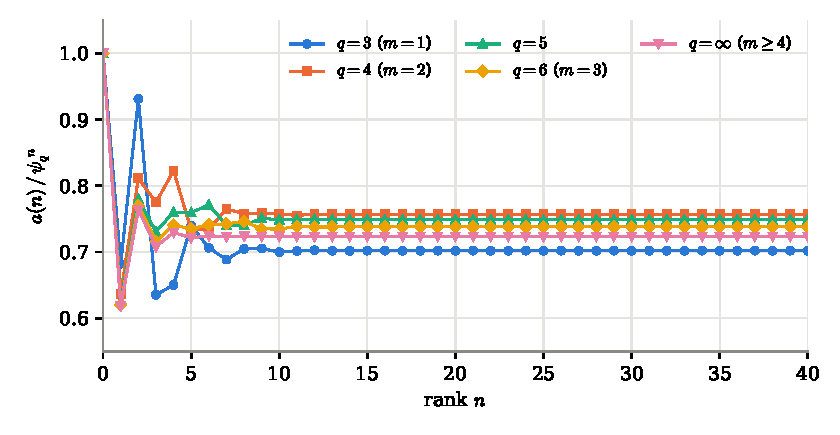
\includegraphics[width=0.84\textwidth]{figures/growth.pdf}
\caption{The normalized counts $a_q(n)/\psi_q^{\,n}$ for $0\le n\le40$. Each sequence tends to the
constant $C_q$ of Table~\ref{tab:growth}.}
\label{fig:growth}
\end{figure}

\begin{remark}\label{rem:nearest}
For $q=3$, \cite[Proposition~5.2]{P137} gives the error term $O(\psi^{-n/2})$. For $q\ge4$ the other
roots of $D_q$ are only a little outside the unit circle (the smallest moduli are $1.0999$, $1.0556$
and $1.0343$ for $q=4,5,6$), so the error term decays slowly. We checked with $40$-digit arithmetic
that $a_q(n)$ is the nearest integer to $C_q\psi_q^{\,n}$ for $1\le n\le80$ and $q=3,4,5,6$. For
$q=3,4,6$ we also bounded the error by $E(n)=\sum_i|c_i|\,|t_i|^{-n}$, where the $c_i$ are the
partial fraction coefficients at the other roots $t_i$ of $D_q$. This bound decreases in $n$, and it
is below $\tfrac12$ for $n\ge3$, $n\ge6$ and $n\ge11$ when $q=3$, $4$ and $6$. Together with the
direct check, this gives the rounding for every $n\ge1$ when $q=3,4,6$. These are computer checks in
$40$-digit floating point, not in interval arithmetic, so they are not proofs.
\end{remark}

\section{The free case \texorpdfstring{$m\ge4$}{m >= 4}}\label{sec:free}

For $m\ge4$ the map $g_m\circ f$ has infinite order (Lemma~\ref{lem:order}), so there is no relation
to shorten words, and every string is reduced. We work directly in $x$-coordinates. Call a string
$(c_1,\dots,c_k)$ with $k\ge1$, $c_1\ge0$ and $c_2,\dots,c_k\ge1$ a \emph{free string}. Its value is
\[
x=c_1+g_m\Bigl(c_2+g_m\bigl(c_3+\dots+g_m(c_k)\bigr)\Bigr),
\]
its tails are $T_j=c_j+g_m(T_{j+1})$ with $T_k=c_k$, and its weight is $c_1+\dots+c_k+k-1$.

\begin{theorem}[Theorem~E]\label{thm:free}
Let $m\ge4$, $f(x)=x+1$ and $g_m(x)=-1/(mx)$.
\begin{enumerate}[(a)]
\item Every tail $T_j$ with $j\ge2$ of a free string is greater than $\tfrac12$, so $g_m$ is never applied
at $0$. A free string with $c_1\ge1$ has value in $(c_1-2/m,\,c_1]$, and one with $c_1=0$ and $k\ge2$ has
value in $(-2/m,\,0)$. Distinct free strings have distinct values.
\item The points of the $m$-tree are exactly the values of free strings, and the rank of a point is the
weight of its string.
\item $a(n)=F_{n+1}$ for every $n\ge0$, and the number of positive points of rank $n\ge1$ is $F_n$.
The generating function is $1/(1-t-t^2)$.
\item A vertex is blue if and only if it is negative, and every point has exactly one shortest word.
\item No rational in $(-\infty,-2/m]$ is in the tree, and for each integer $c\ge1$ no rational in
$(c-1,\,c-2/m]$ is in the tree. In particular $-1$ and $\tfrac12$ are never reached.
\end{enumerate}
\end{theorem}

\begin{proof}
(a) First $T_k=c_k\ge1>\tfrac12$. If $T>\tfrac12$ and $c\ge1$, then
$c+g_m(T)=c-1/(mT)>1-2/m\ge\tfrac12$. By downward induction every tail $T_j$ with $j\ge2$ is greater
than $\tfrac12$, and in particular $g_m$ is applied only at positive numbers. For $k\ge2$ the value is
$c_1-1/(mT_2)$ with $0<1/(mT_2)<2/m$, which gives the two intervals. For $k=1$ the value is $c_1$.
Since $2/m\le\tfrac12<1$, the intervals $(c-2/m,c]$ for $c=1,2,\dots$ and $(-2/m,0)$ are disjoint,
and none contains $0$. So the value $x$ decides whether $c_1=0$, and if $c_1\ge1$ then
$c_1=\lceil x\rceil$, and $k=1$ exactly when $x$ is an integer. When $k\ge2$ the tail value $T_2$ is
$g_m(x-c_1)$. So the value determines $c_1$, whether $k=1$, and $T_2$, and induction on $k$ shows that
distinct free strings have distinct values. The string $(0)$ has the value $0$.

(b) Let $V$ be the set of values and $W(x)$ the weight of the string of $x\in V$. Each string is a word
of length $W(x)$ that reaches $x$, so $d\le W$ on $V$. Next, $V$ is closed under the moves, and each
move raises $W$ by at most $1$. Indeed, $f(0)=1$ has the string $(1)$. If $y>0$ has the string
$(c_1,\dots,c_k)$, then $f(y)$ has the string $(c_1+1,c_2,\dots,c_k)$ and $g_m(y)$ has the string
$(0,c_1,\dots,c_k)$, both of weight $W(y)+1$. If $y<0$ has the string $(0,c_2,\dots,c_k)$, then
$g_m(y)$ is the value of $(c_2,\dots,c_k)$, of weight $W(y)-1$, and $f(y)$ has the string
$(1,c_2,\dots,c_k)$, of weight $W(y)+1$. Since $W(0)=0$, every point reached by $n$ moves lies in $V$
and has $W\le n$. So the tree is $V$ and $d=W$.

(c) For the positive points, $c_1\ge1$ contributes $t/(1-t)$, and each later digit $c\ge1$ together
with its $g_m$ contributes $t^{c+1}$, which sums to $t^2/(1-t)$. So
\[
\sum_{n\ge1}r(n)\,t^n=\frac{t}{1-t}\cdot\frac{1}{1-t^2/(1-t)}=\frac{t}{1-t-t^2}.
\]
The map $g_m$ is a bijection from the positive points of rank $n-1$ onto the negative points of rank
$n$, by (b), since $g_m(y)$ has the string $(0,c_1,\dots,c_k)$. So
$\sum_n a(n)t^n=1+(1+t)t/(1-t-t^2)=1/(1-t-t^2)$.

(d) Let $x<0$ be in the tree. Its in-neighbors are $x-1$ and $g_m(x)$. Since $x-1<-1\le-2/m$, the
point $x-1$ is not in the tree by (a) and (b). So the last move of every path to $x$ is $g_m$. Let
$x>0$. Its in-neighbors are $x-1$ and $g_m(x)$, and $g_m(x)$ has rank $d(x)+1$ by the proof of (c).
So the last move of a shortest path to $x$ is $f$. Uniqueness of the shortest word follows by
induction on the rank.

(e) This is (a) and (b). Note that $-1\le-2/m$, and $\tfrac12\in(0,1-2/m]$ since $m\ge4$.
\end{proof}

For $m=4$ the parent map of Section~\ref{sec:parent} does not terminate everywhere. It sends
$\tfrac12$ to $-\tfrac12$ and $-\tfrac12$ back to $g_4(-\tfrac12)=\tfrac12$, and both points are
outside the tree by (e). With $x=ky$, the tree of $x\mapsto x+k$ and $x\mapsto-1/x$ is the $k^2$-tree,
so Theorem~E applies to it for every $k\ge2$.

\section{Computational verification}\label{sec:verify}

The proofs above do not depend on any computation. As a check, the script
\texttt{verify\_general.py} (Python with the standard \texttt{fractions} module, \texttt{sympy} for the
transfer matrix, and \texttt{mpmath} with $40$ digits for the constants of Table~\ref{tab:growth}, about
five minutes) recomputes every
number in this paper by two independent methods. The first is breadth-first search from $0$ in exact
arithmetic, which is Kimberling's row construction. The second enumerates the reduced strings of
Theorem~\ref{thm:Bq} and evaluates each word at $0$. Rationals are Python fractions, and the
$\lambda_5$-tree uses exact arithmetic in $\Q(\sqrt5)$ with $\lambda_5=(1+\sqrt5)/2$. The script checks the
following, and none of the checks fails.

\begin{enumerate}[itemsep=1pt,topsep=3pt]
\item For $m=1$ to rank $24$ ($21{,}304$ points), $m=2$ to rank $28$ ($638{,}804$ points), $m=3$ to
rank $30$ ($3{,}228{,}541$ points), $q=5$ to rank $20$ ($24{,}514$ points) and $m=4,5,6$ to rank $22$
($75{,}024$ points each), the two methods give the same points with the same ranks. No reduced word
applies $g$ at $0$, no two reduced strings have the same value, and every point found by the search
has a reduced string. The counts equal the coefficients of $N_q/D_q$, or of $1/(1-t-t^2)$ in the free
case.
\item In the same ranges, the recurrence of Theorem~\ref{thm:Aq} holds from $n=2q-2$ on and fails at
$n=2q-3$ with defect $-1$, and $a(n)=r(n)+r(n-1)$.
\item At every point found by the search, the parent map, run from the value alone, reaches $0$ in
exactly $d(x)$ steps, and the digits it reads off equal the reduced string. Each point is reached at
its rank by exactly one edge, and it is reached by $g$ exactly when it is negative. For $x<-1$ in range,
$d(x+1)=d(x)-(2q-3)$, and $d(-1)=2q-4$.
\item For $m=1,2,3$ the parent map reaches $0$ from all $4{,}407$ rationals $u/v$ with $|u|,v\le60$, and
for $m=4$ it fails from $3{,}726$ of them. The identities $h(x+1)=h(x)$ and $h(g_m(x))=mx^2h(x)$ of the
proof of Theorem~\ref{thm:reach} hold for $|u|,v\le200$. For $m=4,5,6$ the points lie in the intervals of
Theorem~\ref{thm:free}(a), and $-1$ and $\tfrac12$ are not reached.
\item A transfer matrix for the run rule, solved symbolically, gives the generating function $N_q/D_q$
with $\gcd(N_q,D_q)=1$ for $3\le q\le8$, without using the formula of Theorem~\ref{thm:Aq}.
\item The constants of Table~\ref{tab:growth} agree when computed from the residue
$-N_q(t_0)/(t_0D_q'(t_0))$, from the formula of Proposition~\ref{prop:growth}, and from
$a_q(400)/\psi_q^{400}$. Every other root of $D_q$ has modulus greater than $1$. Remark~\ref{rem:nearest}
is checked here.
\item Table~\ref{tab:hand}, the examples, the identity with A060961 for $1\le n\le21$, and the
numbers of vertices in Figure~\ref{fig:trees} ($31$ and $48$).
\end{enumerate}

Table~\ref{tab:counts} lists the first counts. The script \texttt{make\_figures.py} draws
Figures~\ref{fig:trees} and~\ref{fig:growth}.

\begin{table}[ht]
\centering\small
\begin{tabular}{@{}r r r r r r@{}}
\toprule
$n$ & $q=3$ ($m=1$) & $q=4$ ($m=2$) & $q=5$ & $q=6$ ($m=3$) & $q=\infty$ ($m\ge4$)\\
\midrule
0 & 1 & 1 & 1 & 1 & 1\\
1 & 1 & 1 & 1 & 1 & 1\\
2 & 2 & 2 & 2 & 2 & 2\\
3 & 2 & 3 & 3 & 3 & 3\\
4 & 3 & 5 & 5 & 5 & 5\\
5 & 5 & 7 & 8 & 8 & 8\\
6 & 7 & 11 & 13 & 13 & 13\\
7 & 10 & 18 & 20 & 21 & 21\\
8 & 15 & 28 & 32 & 34 & 34\\
9 & 22 & 44 & 52 & 54 & 55\\
10 & 32 & 69 & 83 & 87 & 89\\
11 & 47 & 108 & 133 & 141 & 144\\
12 & 69 & 170 & 213 & 227 & 233\\
13 & 101 & 267 & 341 & 366 & 377\\
14 & 148 & 419 & 546 & 590 & 610\\
15 & 217 & 658 & 874 & 951 & 987\\
16 & 318 & 1{,}033 & 1{,}400 & 1{,}533 & 1{,}597\\
17 & 466 & 1{,}622 & 2{,}242 & 2{,}471 & 2{,}584\\
18 & 683 & 2{,}547 & 3{,}590 & 3{,}983 & 4{,}181\\
19 & 1{,}001 & 3{,}999 & 5{,}749 & 6{,}420 & 6{,}765\\
20 & 1{,}467 & 6{,}279 & 9{,}206 & 10{,}349 & 10{,}946\\
\bottomrule
\end{tabular}
\caption{The counts $a_q(n)$ for $0\le n\le20$. The columns for $q=3,4,6$ count rationals, the column
for $q=5$ counts points of $\Q(\sqrt5)$, and the last column is the Fibonacci numbers $F_{n+1}$.}
\label{tab:counts}
\end{table}

\section{Related work and open questions}\label{sec:final}

\paragraph{Related work.} The groups $H_q=\langle F,G\rangle$ were defined by Hecke \cite{hecke1936}, and
the continued fractions of Section~\ref{sec:words} go back to Rosen \cite{rosen1954}. The full texts of
these two papers were not available to us, and we rely on the later sources cited here for their
content. Rosen's fractions, as described in \cite[Section~1.2]{rosen-schmidt} and \cite{short-walker},
use the nearest multiple of $\lambda$ and digits of both signs, so his normal form is not ours. The closest work
we know is by Short and Walker \cite{short-walker}. They show that Rosen fractions correspond to paths in
a Farey-type graph and characterize the \emph{geodesic} expansions, those with the fewest terms, by
forbidden blocks of digits \cite[Theorem~1.3 for even $q$ and Theorem~7.1 for odd $q$]{short-walker}. Their condition and our run rule both come
from the relation $(GF)^q=\mathrm{id}$. But they count terms and allow digits of both signs, while we
count moves and use only forward moves, so the forbidden blocks differ. For example, for $q=6$ they
forbid three consecutive digits $1$ and we forbid four. Janvresse, Rittaud and de la Rue study the
positive all-minus $\lambda$-fractions of Section~\ref{sec:words} as a dynamical system conjugate to a
$\beta$-shift \cite{jrr}. Their count is by number of digits, which gives a different sequence. Taha
builds a Stern--Brocot process for the Hecke groups \cite{taha}, which inserts mediants and does not
count by word length.

For free products there is a classical formula for growth series \cite{paris-varghese}, but it needs a
generating set that is a union of generating sets of the factors. Our generators $f$ and $g$ are not of
that form, since $f=g\circ(g\circ f)$ mixes the two factors. Also we use only forward moves, and we
count points, not group elements.

Kimberling and Moses \cite{kimberling-moses} studied several trees of this kind. Their Theorem~3.2 shows
that the tree of $x\mapsto x+k$ and $x\mapsto k/x$ with root $1$ has Fibonacci counts. Their
Example~4.2 states the recurrence $a(n)=a(n-1)+a(n-3)$ for the tree of $x+1$ and $-1/x$ with root
$1$. Their Example~4.4, with $x\mapsto x+1$ and $x\mapsto-m/x$, is not in our family, since there the
composite has trace squared over determinant equal to $1/m$, which is not $4\cos^2(\pi/q)$ for any $q$.

As far as we know, the counts $a(n)$ for $m=2$ and $m=3$, the run rule, Theorem~D, and the fact that the
rank generating function depends only on $q$ are new. The group theory around them is classical.

\paragraph{The cusp set.} By Proposition~\ref{prop:closed}(d), the $\lambda_q$-tree is the orbit of
$\infty$ under $H_q$ with $\infty$ removed, since $G(\infty)=0$. This orbit is the set of cusps of $H_q$.
For $q=5,8,10,12$, Leutbecher showed that the cusps are $\lambda_q\Q(\lambda_q^2)$ together with $\infty$
(Satz~2, as stated in the introduction of \cite{leutbecher1974}). Winsor also attributes this case to
Leutbecher and McMullen \cite{winsor}. Hence the $\lambda_5$-tree is
all of $\Q(\sqrt5)$. For most $q\ge7$ the cusp set is not known \cite{rosen-schmidt,winsor}. Our
Theorems~A$_q$, B$_q$ and C$_q$ hold for every $q$ all the same, because they never use the cusp set.

\paragraph{Open questions.}
\begin{enumerate}[itemsep=2pt,topsep=3pt]
\item \emph{Other involutions.} Any rational M\"obius involution $g(x)=(ax+b)/(cx-a)$ can be paired with
$f(x)=x+1$. Then $g\circ f$ has trace $c$ and determinant $-(a^2+bc)$, and it has finite order $q$
exactly when $c^2/(-(a^2+bc))$ is $0$, $1$, $2$ or $3$, with $q=2,3,4,6$, assuming $-(a^2+bc)>0$. Is the rank generating function
then always $N_q/D_q$, perhaps up to a correction at the root? A fixed point of $g$ or a pole inside
the tree may change the small ranks.
\item \emph{The free case.} Describe exactly which rationals the $m$-tree reaches for $m\ge4$.
Theorem~\ref{thm:free} gives only necessary conditions.
\item \emph{Rounding.} Prove that $a_q(n)$ is the nearest integer to $C_q\psi_q^{\,n}$ for every $n\ge1$
and every $q$, or give a rigorous proof for $q=4,6$ (Remark~\ref{rem:nearest}).
\item \emph{Ordinary continued fractions.} For $q=3$ the rank also has a formula in terms of the
ordinary continued fraction \cite[Theorem~4.8]{P137}. Is there a similar formula for $m=2$ and $m=3$?
\item \emph{The constants.} Is there a closed form for the share of negative points, or for $C_q$, that
explains why $C_q$ is not monotone in $q$?
\end{enumerate}

\subsection*{Data and code availability}
The scripts \texttt{verify\_general.py} and \texttt{make\_figures.py} are in the repository
\url{https://github.com/apemm/Kagey-Problems}, in the folder\\
\texttt{kagey-problems/problem137/general}.


\paragraph{Acknowledgment.} I thank Peter Kagey for posing the problem.

\section*{A note on the use of AI}
The following ideas were suggested by an AI model (Claude, made by Anthropic, model Opus 5.5, used
through Claude Code in October 2026). These are the generalization to $x\mapsto-1/(mx)$, the reading of
the $3$ in Problem 137 as the order of $g\circ f$, the run rule of Theorem~B$_q$, the reduction of
$x\mapsto x+k$ with $x\mapsto-1/x$ to the case $m=k^2$, the title, the directions on $q=5$ and on
the growth constants $\psi_q$ and $C_q$, the question on other involutions, and a proof route
through normal forms in free products that this paper does not use (Remark~\ref{rem:relation}). The
model also wrote the verification scripts \texttt{verify\_general.py} and \texttt{make\_figures.py},
and it drafted the proofs, the literature survey and the text, which the author then revised. I checked the proofs by prompting the same model
to audit their logic line by line in separate passes. Every count and every rank in the paper was
also checked by computer, to depth 28 for $m=2$ and 30 for $m=3$, by two independent methods
(\texttt{verify\_general.py}). All claims and proofs in this paper are the responsibility of the
author.

\begin{thebibliography}{99}\small\setlength{\itemsep}{1pt}

\bibitem{fairchild-hanusa}
S.~Fairchild and C.~R.~H.~Hanusa, Densities of arithmetic Hecke triangle group orbits, preprint,
2026, \url{https://arxiv.org/abs/2607.22142}.

\bibitem{hecke1936}
E.~Hecke, \"Uber die Bestimmung Dirichletscher Reihen durch ihre Funktionalgleichung,
\emph{Math.\ Ann.} \textbf{112} (1936), 664--699.

\bibitem{im-lee}
B.-H.~Im and W.~Lee, Non-holomorphic Eisenstein series for certain Fuchsian groups and class numbers,
preprint, 2022, \url{https://arxiv.org/abs/2207.05325}.

\bibitem{jrr}
E.~Janvresse, B.~Rittaud, and T.~de~la~Rue, Dynamics of $\lambda$-continued fractions and
$\beta$-shifts, preprint, 2011, \url{https://arxiv.org/abs/1103.6181}.

\bibitem{kagey137}
P.~Kagey, Problem 137, Open Problem Collection, \url{https://peterkagey.com/problems/137/}.

\bibitem{kagey-mse}
P.~Kagey, Enumerating all fractions by $x\mapsto x+1$ and $x\mapsto-\frac1x$, Mathematics Stack
Exchange, question 5057812, April 2025, \url{https://math.stackexchange.com/q/5057812}.

\bibitem{kimberling-moses}
C.~Kimberling and P.~J.~C.~Moses, The infinite Fibonacci tree and other trees generated by rules,
\emph{Fibonacci Quart.} \textbf{52} (2014), no.~5, 136--150.

\bibitem{leutbecher1974}
A.~Leutbecher, \"Uber die Heckeschen Gruppen $G(\lambda)$. II, \emph{Math.\ Ann.} \textbf{211}
(1974), 63--86.

\bibitem{mmz}
mathmasterzach, Answer to ``Enumerating all fractions by $x\mapsto x+1$ and $x\mapsto-\frac1x$'',
Mathematics Stack Exchange, April 2025, \url{https://math.stackexchange.com/a/5058406}.

\bibitem{oeisA060961}
OEIS Foundation Inc., Sequence A060961, The On-Line Encyclopedia of Integer Sequences,
\url{https://oeis.org/A060961}.

\bibitem{oeisA226247}
C.~Kimberling, Sequence A226247, The On-Line Encyclopedia of Integer Sequences, 2013,
\url{https://oeis.org/A226247}.

\bibitem{oeisA293506}
OEIS Foundation Inc., Sequence A293506, The On-Line Encyclopedia of Integer Sequences,
\url{https://oeis.org/A293506}.

\bibitem{paris-varghese}
L.~Paris and O.~Varghese, The growth series of Dyer groups, preprint, 2023,
\url{https://arxiv.org/abs/2305.09796}.

\bibitem{P137}
A.~Pemmasani, The tree of rationals generated by $x\mapsto x+1$ and $x\mapsto-1/x$: an exact distance
formula and the rank recurrence, preprint, 2026.

\bibitem{rosen1954}
D.~Rosen, A class of continued fractions associated with certain properly discontinuous groups,
\emph{Duke Math.\ J.} \textbf{21} (1954), 549--563.

\bibitem{rosen-schmidt}
D.~Rosen and T.~A.~Schmidt, Hecke groups and continued fractions, \emph{Bull.\ Austral.\ Math.\ Soc.}
\textbf{46} (1992), 459--474.

\bibitem{short-walker}
I.~Short and M.~Walker, Geodesic Rosen continued fractions, \emph{Q.\ J.\ Math.} \textbf{67} (2016),
519--549.

\bibitem{taha}
D.~Taha, On cross sections to the geodesic and horocycle flows on quotients of
$\mathrm{SL}(2,\mathbb{R})$ by Hecke triangle groups $G_q$, preprint, 2019,
\url{https://arxiv.org/abs/1906.07250}.

\bibitem{winsor}
K.~Winsor, Hecke triangle groups and special hyperbolic elements, preprint, 2026,
\url{https://arxiv.org/abs/2605.30064}.

\end{thebibliography}


\end{document}
